\chapter{Metodologia e Resultados}
\label{cap:metodologia-e-resultados}

O trabalho foi desenvolvido de acordo coma as etapas apresentados no fluxograma da \autoref{fig:flux-metodologia}.

Visando uma melhor execução, a metodologia \textit{site survey} foi implementada seguindo as respectivas fases:
\begin{compactitem}
	\item \textbf{Reconhecimento do local:} o Bloco Didático foi inspecionado em busca de características estruturais que possam vir a influenciar na propagação do sinal Wi-Fi.
	
	\item \textbf{Coleta de dados:} com o auxílio de \textit{softwares}, medidas de potência foram capturadas em diversos pontos do prédio e posteriormente marcados na planta baixa do prédio.
	
	\item \textbf{Tratamento dos dados:} depois de coletados, os dados foram tratados a fim de filtrar quais seriam úteis para a proposta do trabalho.
	
	\item \textbf{Geração dos mapas de calor:} representações gráficas da cobertura de rádio do ponto de acesso foram feitas para demonstrar onde o sinal sofria maiores perdas.
\end{compactitem}

\begin{figure}[H]
	\centering
	\Caption{\label{fig:flux-metodologia}Fluxograma da metodologia do trabalho.}	
	\UECEfig{}{
		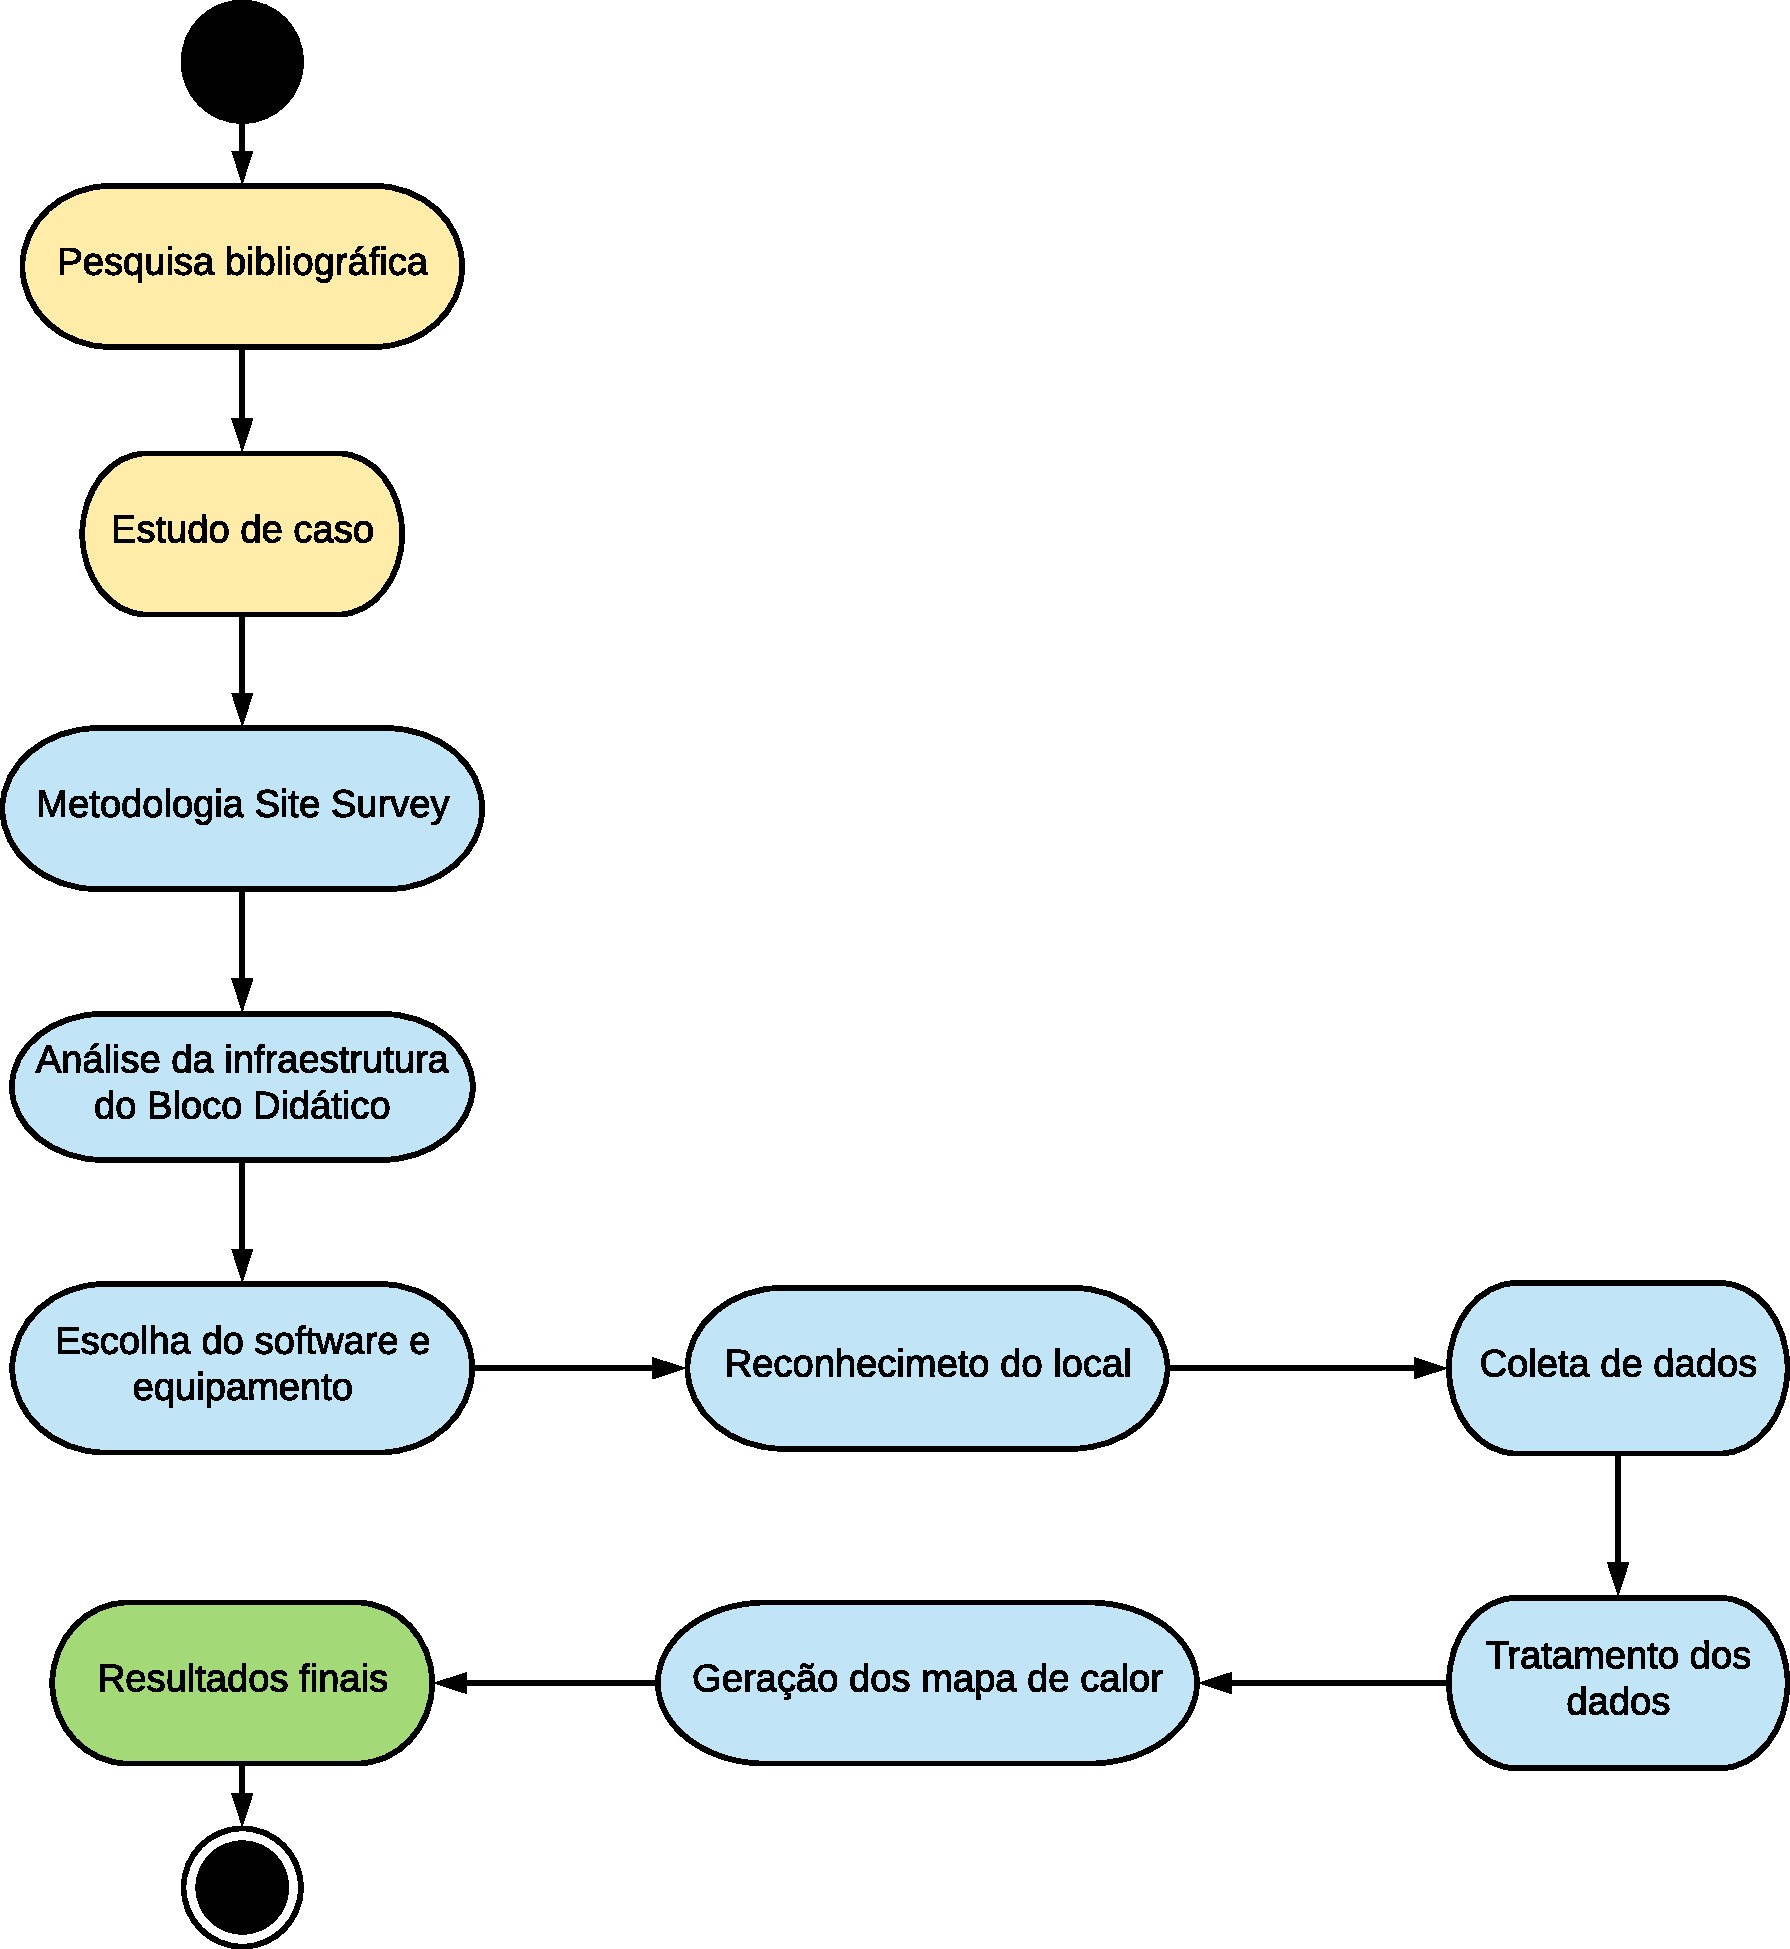
\includegraphics[scale=.38]{figuras/fluxograma_metodologia_tcc_01.pdf}
	}{
		\Fonte{Autor.}%
	}	
\end{figure}

\section{Estudo de Caso}
\label{sec:estudo-de-caso}

O Instituto Federal de Educação, Ciência e Tecnologia do Ceará conta com 32 \textit{campi} em funcionamento distribuídos por todo o estado. O \textit{campus} de Tauá do IFCE, foi inaugurado em 20 de novembro de 2009. O \textit{campus} abrange principalmente os municípios de Aiuaba, Arneiroz, Quiterianópolis e Parambu, e recebe alunos de várias outras regiões por meio do Sistema de Seleção Unificada (SISU) do Ministério da Educação (MEC) \cite{ifceTaua2019}.

O \textit{campus} Tauá oferta atualmente os cursos técnicos integrados em Redes de Computadores e Agropecuária e os cursos superiores de Tecnologia de Telemática e Licenciatura em Letras com habilitação em Inglês e Português. No semestre letivo 2019.1, o \textit{campus} conta com mais de 400 alunos matriculados \cite{ifceTaua2019}.

A estrutura física do IFCE Tauá pode ser dividida em duas partes principais: a primeira conta com a instalação original do projeto (inaugurada em 2009), onde está inserida a administração, os laboratórios e a biblioteca; a segunda representa o Bloco Didático, inaugurado em 5 de julho de 2016, o qual abriga nove salas de aula, a coordenadoria de cursos e os laboratórios de informática e eletromagnetismo. O presente trabalho foi desenvolvido no Bloco Didático da instituição, já que este concentra as salas de aula, o que resulta em um grande fluxo de pessoas pela área, principalmente de alunos.

O \textit{campus} Tauá conta com diversas atividades de pesquisa, extensão e ensino exercidas por discentes, docentes e técnicos. Assim, a instituição, visando atender a comunidade acadêmica, disponibiliza uma infraestrutura de rede sem fio.

Na \autoref{fig:vista-campus}, tem-se uma visão total da área do \textit{campus}, delimitada pela marcação em vermelho, que é composto pelo bloco inicial do projeto de 2009, destacado em azul, pelo Bloco Didático, em verde, e pela quadra poliesportiva localizada imediatamente acima deste último prédio.

\begin{figure}[H]
	\centering
	\Caption{\label{fig:vista-campus}Visão aérea do IFCE \textit{campus} Tauá.}	
	\UECEfig{}{
		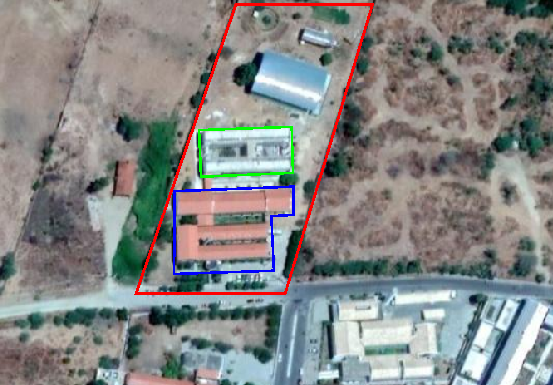
\includegraphics[scale=1]{figuras/ifce-taua-maps.pdf}
	}{
		\Fonte{\citeonline{GoogleMaps}.}
	}	
\end{figure}

%\subsection{Infraestrutura da rede sem fio do IFCE Tauá}
%\label{subsec:infraestrutura-wireless}

A instituição conta com uma infraestrutura de rede sem fio com vários pontos de acesso distribuídos em diversos locais de sua área. No bloco 1 (bloco inicial) encontram-se a maior concentração de pontos de acesso, destinados a suprir as necessidades de conexão à Internet do setor administrativo e de pesquisas desenvolvidas no \textit{campus}. Para o térreo do Bloco Didático, há a presença de dois pontos de acesso: um destinado aos estudantes e o outro aos professores, ambos localizados na sala de coordenação e indicados pelos marcadores conforme ilustra a \autoref{fig:local-ap}. Para o térreo, não existe pontos de acesso instalados. Todos os pontos de acesso no \textit{campus} são protegidos com senhas de acesso alfanuméricos.

\begin{figure}[H]
	\centering
	\Caption{\label{fig:local-ap}Localização dos pontos de acesso no 1º andar do Bloco Didático.}	
	\UECEfig{}{
		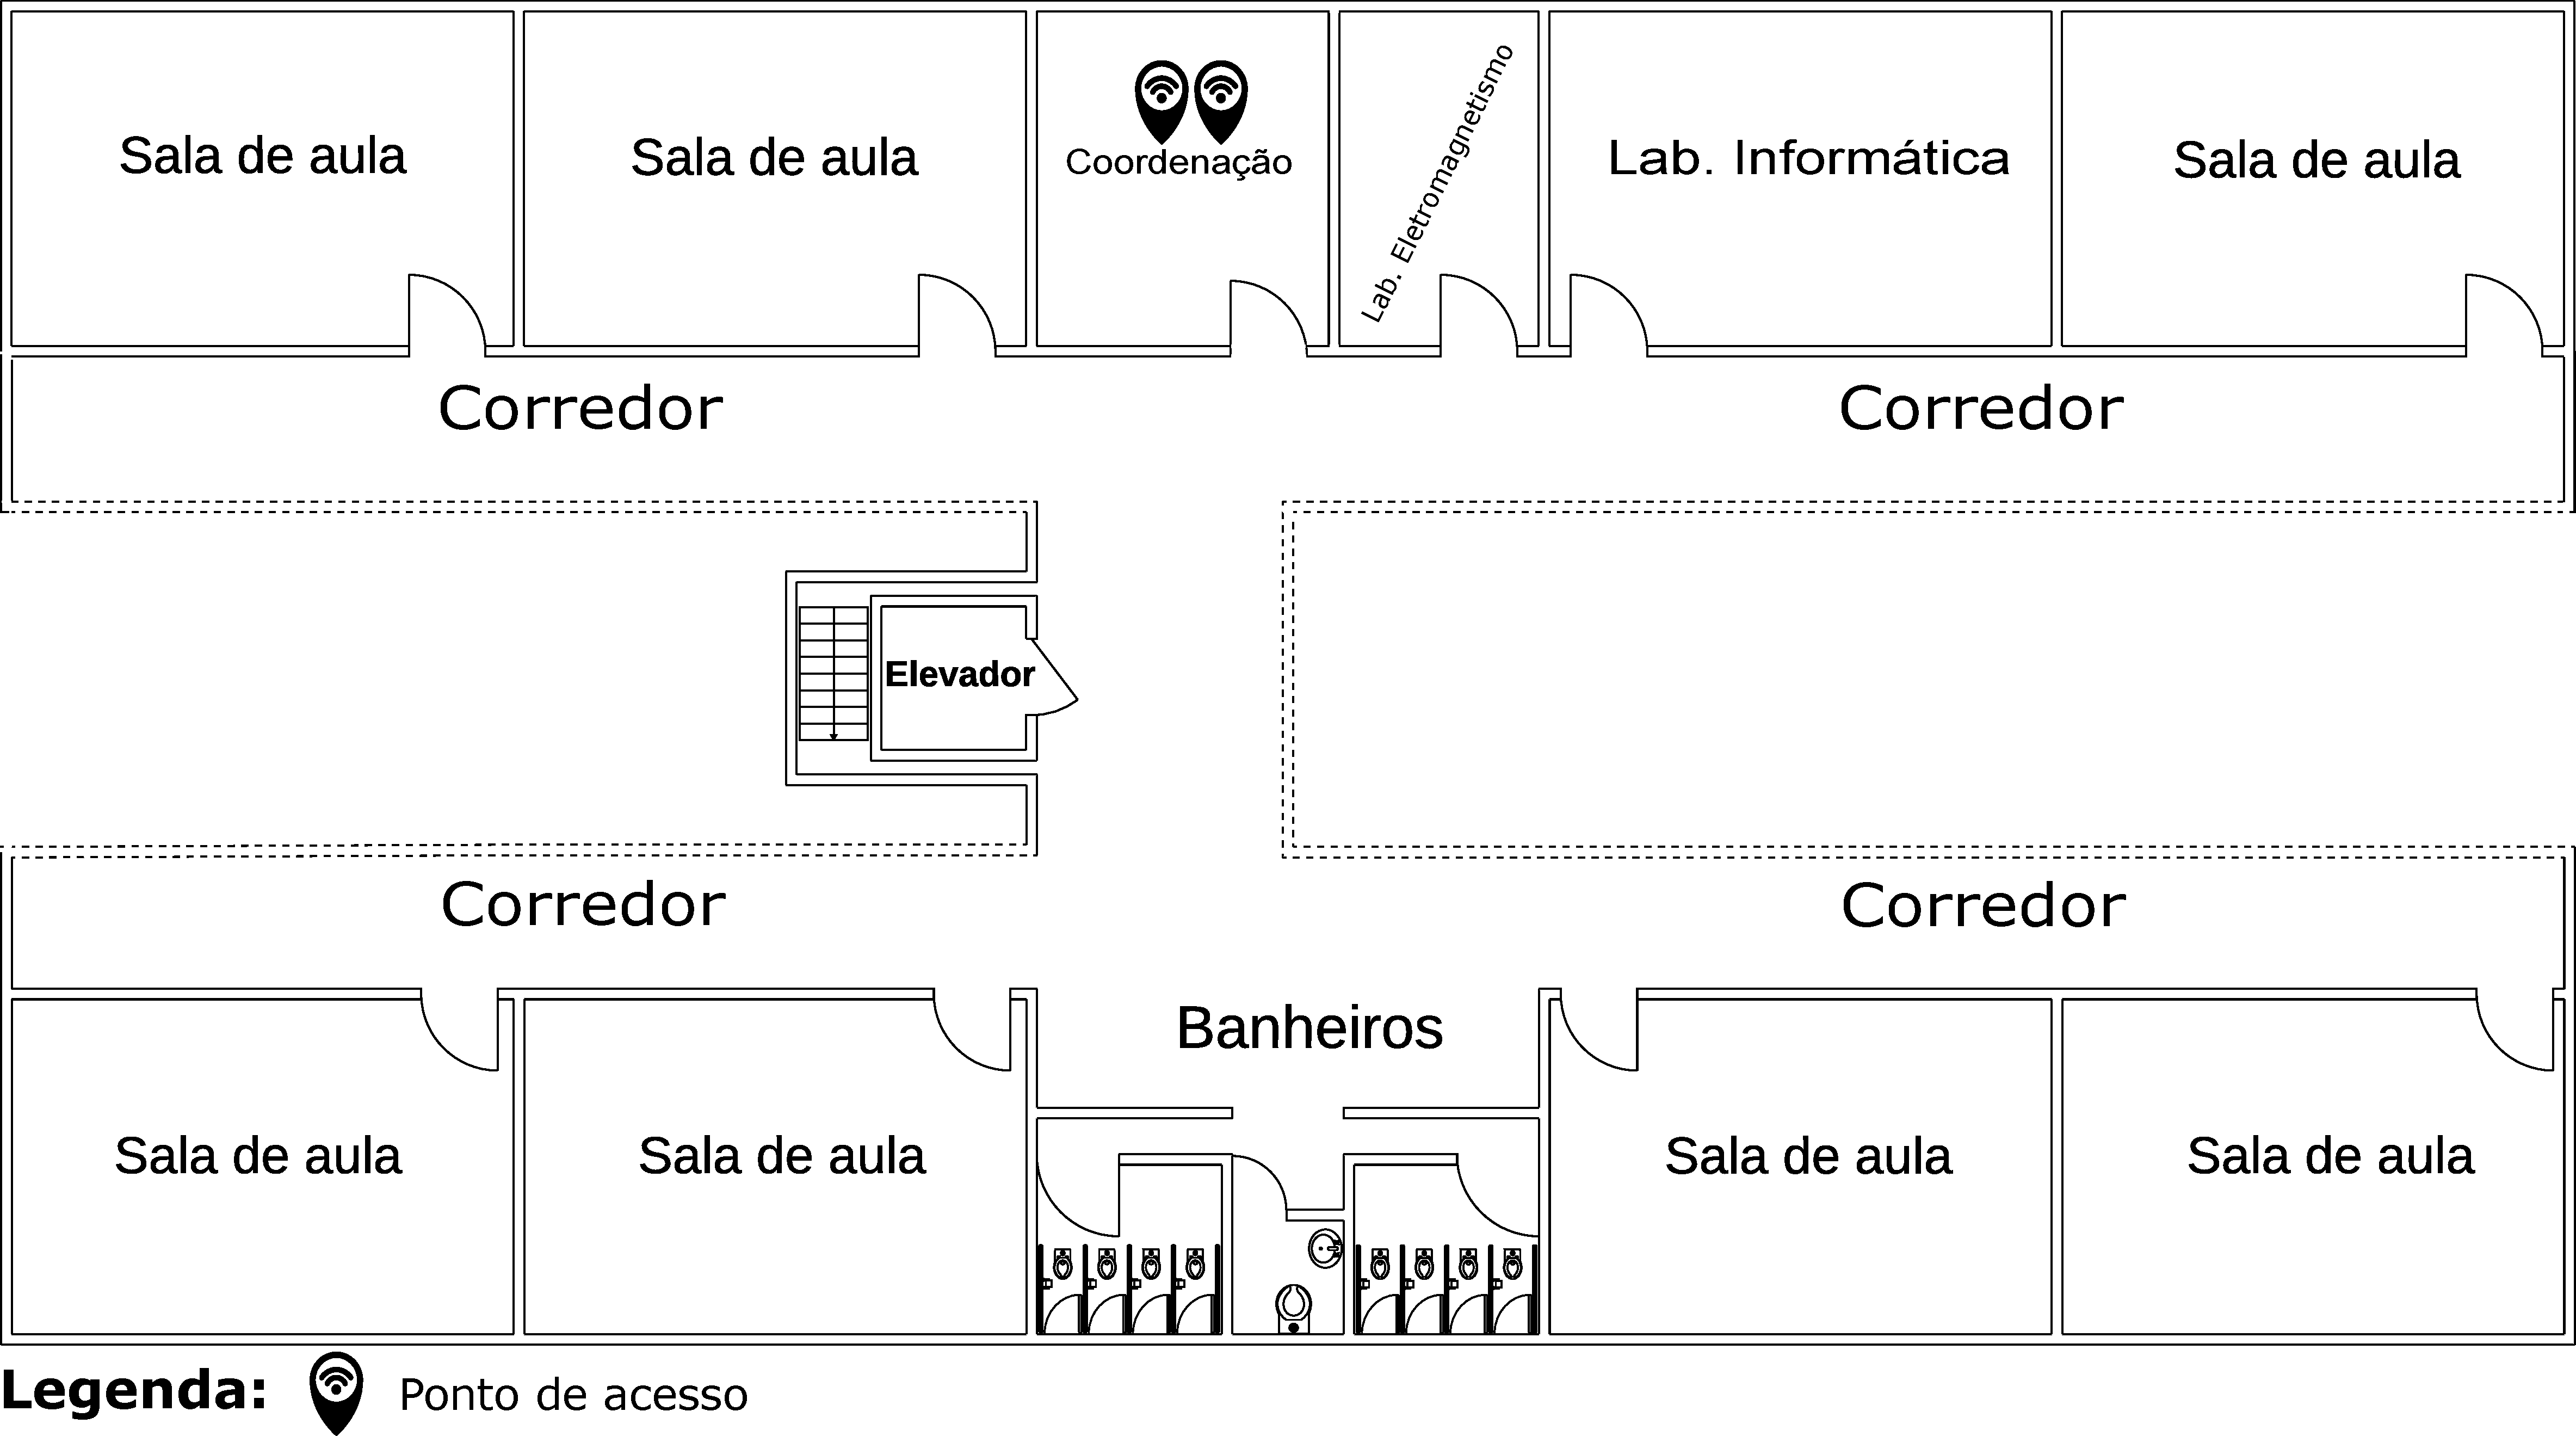
\includegraphics[scale=.18]{figuras/APs_Bloco_Andar_2_02.pdf}
	}{
		\Fonte{Autor.}
	}	
\end{figure}

A Internet disponibilizada no IFCE Tauá é acessível tanto para aqueles que estudam na instituição ou trabalham, como também para visitantes, desde que tenham a senha de acesso. A rede sem fio é dividida de forma a atender cada setor que compõe a organização institucional do \textit{campus}. Isso quer dizer que para os frequentadores da biblioteca existe uma rede específica para eles; para os professores da mesma forma. No entanto, não há restrições para que cada categoria de usuários utilize sua rede própria, cada usuário é livre para associar-se a qualquer ponto de acesso disponível, desde que tenha autorização para tal.

As configurações que podem ser encontradas nos pontos de acesso variam de equipamentos que operam na frequência de 2.4 GHz chegando até ao modo \textit{dual band}.


\section{Materiais utilizados}
\label{materiais-uyilizados}

\subsection{Software}
\label{subsec:softwares-utiliados}

Para que sejam realizados os testes iniciais de \textit{site survey} numa rede sem fio é necessário a utilização de \textit{software(s)} dedicado(s) que permita(m) capturar as informações necessárias que possibilitam avaliar o funcionamento da rede. Neste trabalho foram utilizados dois \textit{softwares}: um para a visualização das redes disponíveis no local alvo (Xirrus Wi-Fi Inspector) e o outro para a geração dos mapas de intensidade de sinal (Ekahau HeatMapper). \textcolor{blue}{A escolha por estes programas se deu pelo fato de serem gratuitos, estáveis, e por não exigirem muitos recursos computacionais.}

Além de ser gratuito, o Xirrus Wi-Fi Inspector apresenta uma interface amigável para a visualização das redes Wi-Fi disponíveis. Além disso, a página principal dele exibe quatros campos diferentes que podem ser expandidos para uma visualização mais detalhada: \textit{Radar}, \textit{History}, \textit{Connection} e \textit{Networks}. Cada um possui algumas funções específicas, mas para a proposta deste trabalho, apenas o campo \textit{Networks} foi explorado, o qual exibe as informações minuciosas das redes detectadas em determinada área (\autoref{fig:software-xirrus}).

\begin{figure}[H]
	\centering
	\Caption{\label{fig:software-xirrus}Tela de \textit{Networks} do Xirrus Wi-Fi Inspector.}	
	\UECEfig{}{
		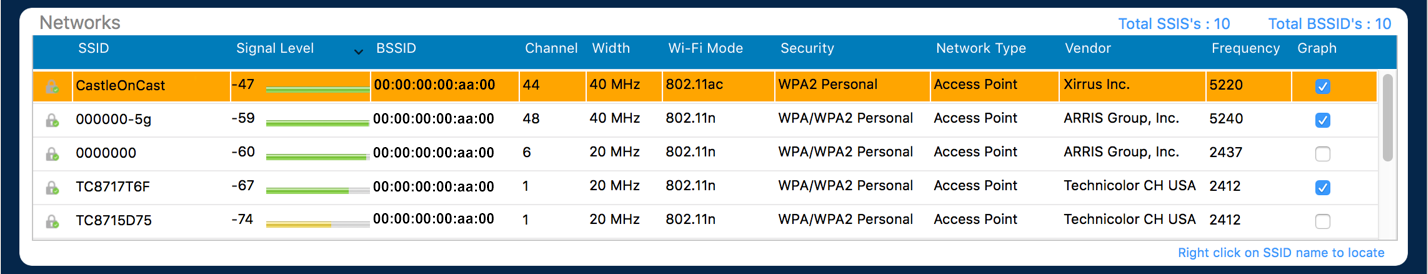
\includegraphics[scale=.41]{figuras/inspector_layout_Riverbed_Networks.png}
	}{
		\Fonte{Autor.}
	}	
\end{figure}

Na janela \textit{Networks} são apresentadas algumas informações dos pontos de acessos descobertos, descritas a seguir:

\begin{compactitem}
	\item \textbf{SSID}: representa o nome da rede sem fio, usado para identificar a mesma, é necessário para associar-se ao ponto de acesso.
	\item \textbf{\textit{Signal Level}:} apresenta a potência do sinal recebido do ponto de acesso em dBm.
	\item \textbf{\textit{Wi-Fi Mode}:} apresenta a versão do padrão 802.11 configurado no ponto de acesso.
	\item \textbf{\textit{Security}:} exibe o protocolo de segurança utilizado pela rede sem fio.
	\item \textbf{\textit{Vendor}:} mostra qual o nome do fabricante do equipamento.
	\item \textbf{BSSID (do inglês, \textit{Basic Service Set Identifier})}: mostra o endereço físico do dispositivo da rede Wi-Fi, que no caso é o endereço MAC (do inglês, \textit{Media Access Control}).
	\item \textbf{\textit{Channel}:} exibe o canal de frequência que o ponto de acesso está utilizando.
	\item \textbf{\textit{Frequency}:} representa a frequência utilizada por um determinado ponto de acesso, podendo ser 2.4 GHz ou 5 GHz.
	\item \textbf{\textit{Network Type}:} exibe o tipo de operação do dispositivo que opera a rede Wi-Fi, seja ponto de acesso ou \textit{ad hoc}.
	\item \textbf{\textit{Graph}:} caixa de seleção para ativar/desativar a representação gráfica do nível de sinal da rede Wi-Fi ao longo do tempo.
\end{compactitem}
	
Já para a criação de mapas de calor dos sinais de radiofrequência, o programa utilizado foi o Ekahau HeatMapper. Com ele é possível descobrir a cobertura de uma rede Wi-Fi padrão 802.11n/b/g a partir da visualização do mapa de calor obtido na coleta de dados em diversos pontos espalhados pelo local.

O programa possibilita ao usuário escolher um arquivo de seu computador que representa a planta baixa do ambiente de interesse, para assim marcar os pontos onde as medidas de potência foram capturadas e posteriormente a coloração. Cada cor exibida pelo \textit{software} significa a intensidade de potência do sinal recebido em certo ponto, variando do verde (sinal forte) até o vermelho (sinal fraco). Além disso, as marcações retilíneas em verde indicam o percurso feito pelo \textit{notebook} durante o mapeamento enquanto os pontos apontam o local de coleta de medidas. Todos esses detalhes são ilustrados pela \autoref{fig:software-ekahau}.

\begin{figure}[H]
	\centering
	\Caption{\label{fig:software-ekahau}Geração do mapa de calor no Ekahau HeatMapper.}	
	\UECEfig{}{
		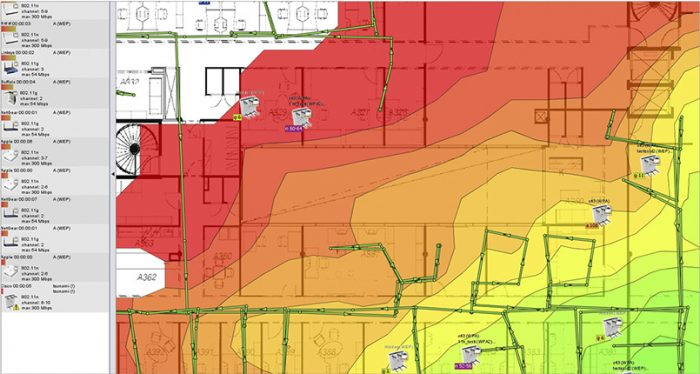
\includegraphics[scale=.5]{figuras/ekahau-heatmapper.jpg}
	}{
		\Fonte{\citeonline{Ekahau2019}.}
	}	
\end{figure}

\subsection{Hardware}
\label{subsec:equipamento-utilizado}

Para poder dar início nas medições dos níveis de potência foi utilizado o \textit{notebook} Positivo Master N40i (\autoref{fig:notebook}) com os \textit{softwares} Xirrus Wi-Fi Inspector e Ekahau HeatMapper instalados e configurados. As especificações do computador podem ser visualizadas na \autoref{tab:carac-notebook}.

\begin{figure}[H]
	\centering
	\Caption{\label{fig:notebook}Notebook Positivo Master N40i.}	
	\UECEfig{}{
		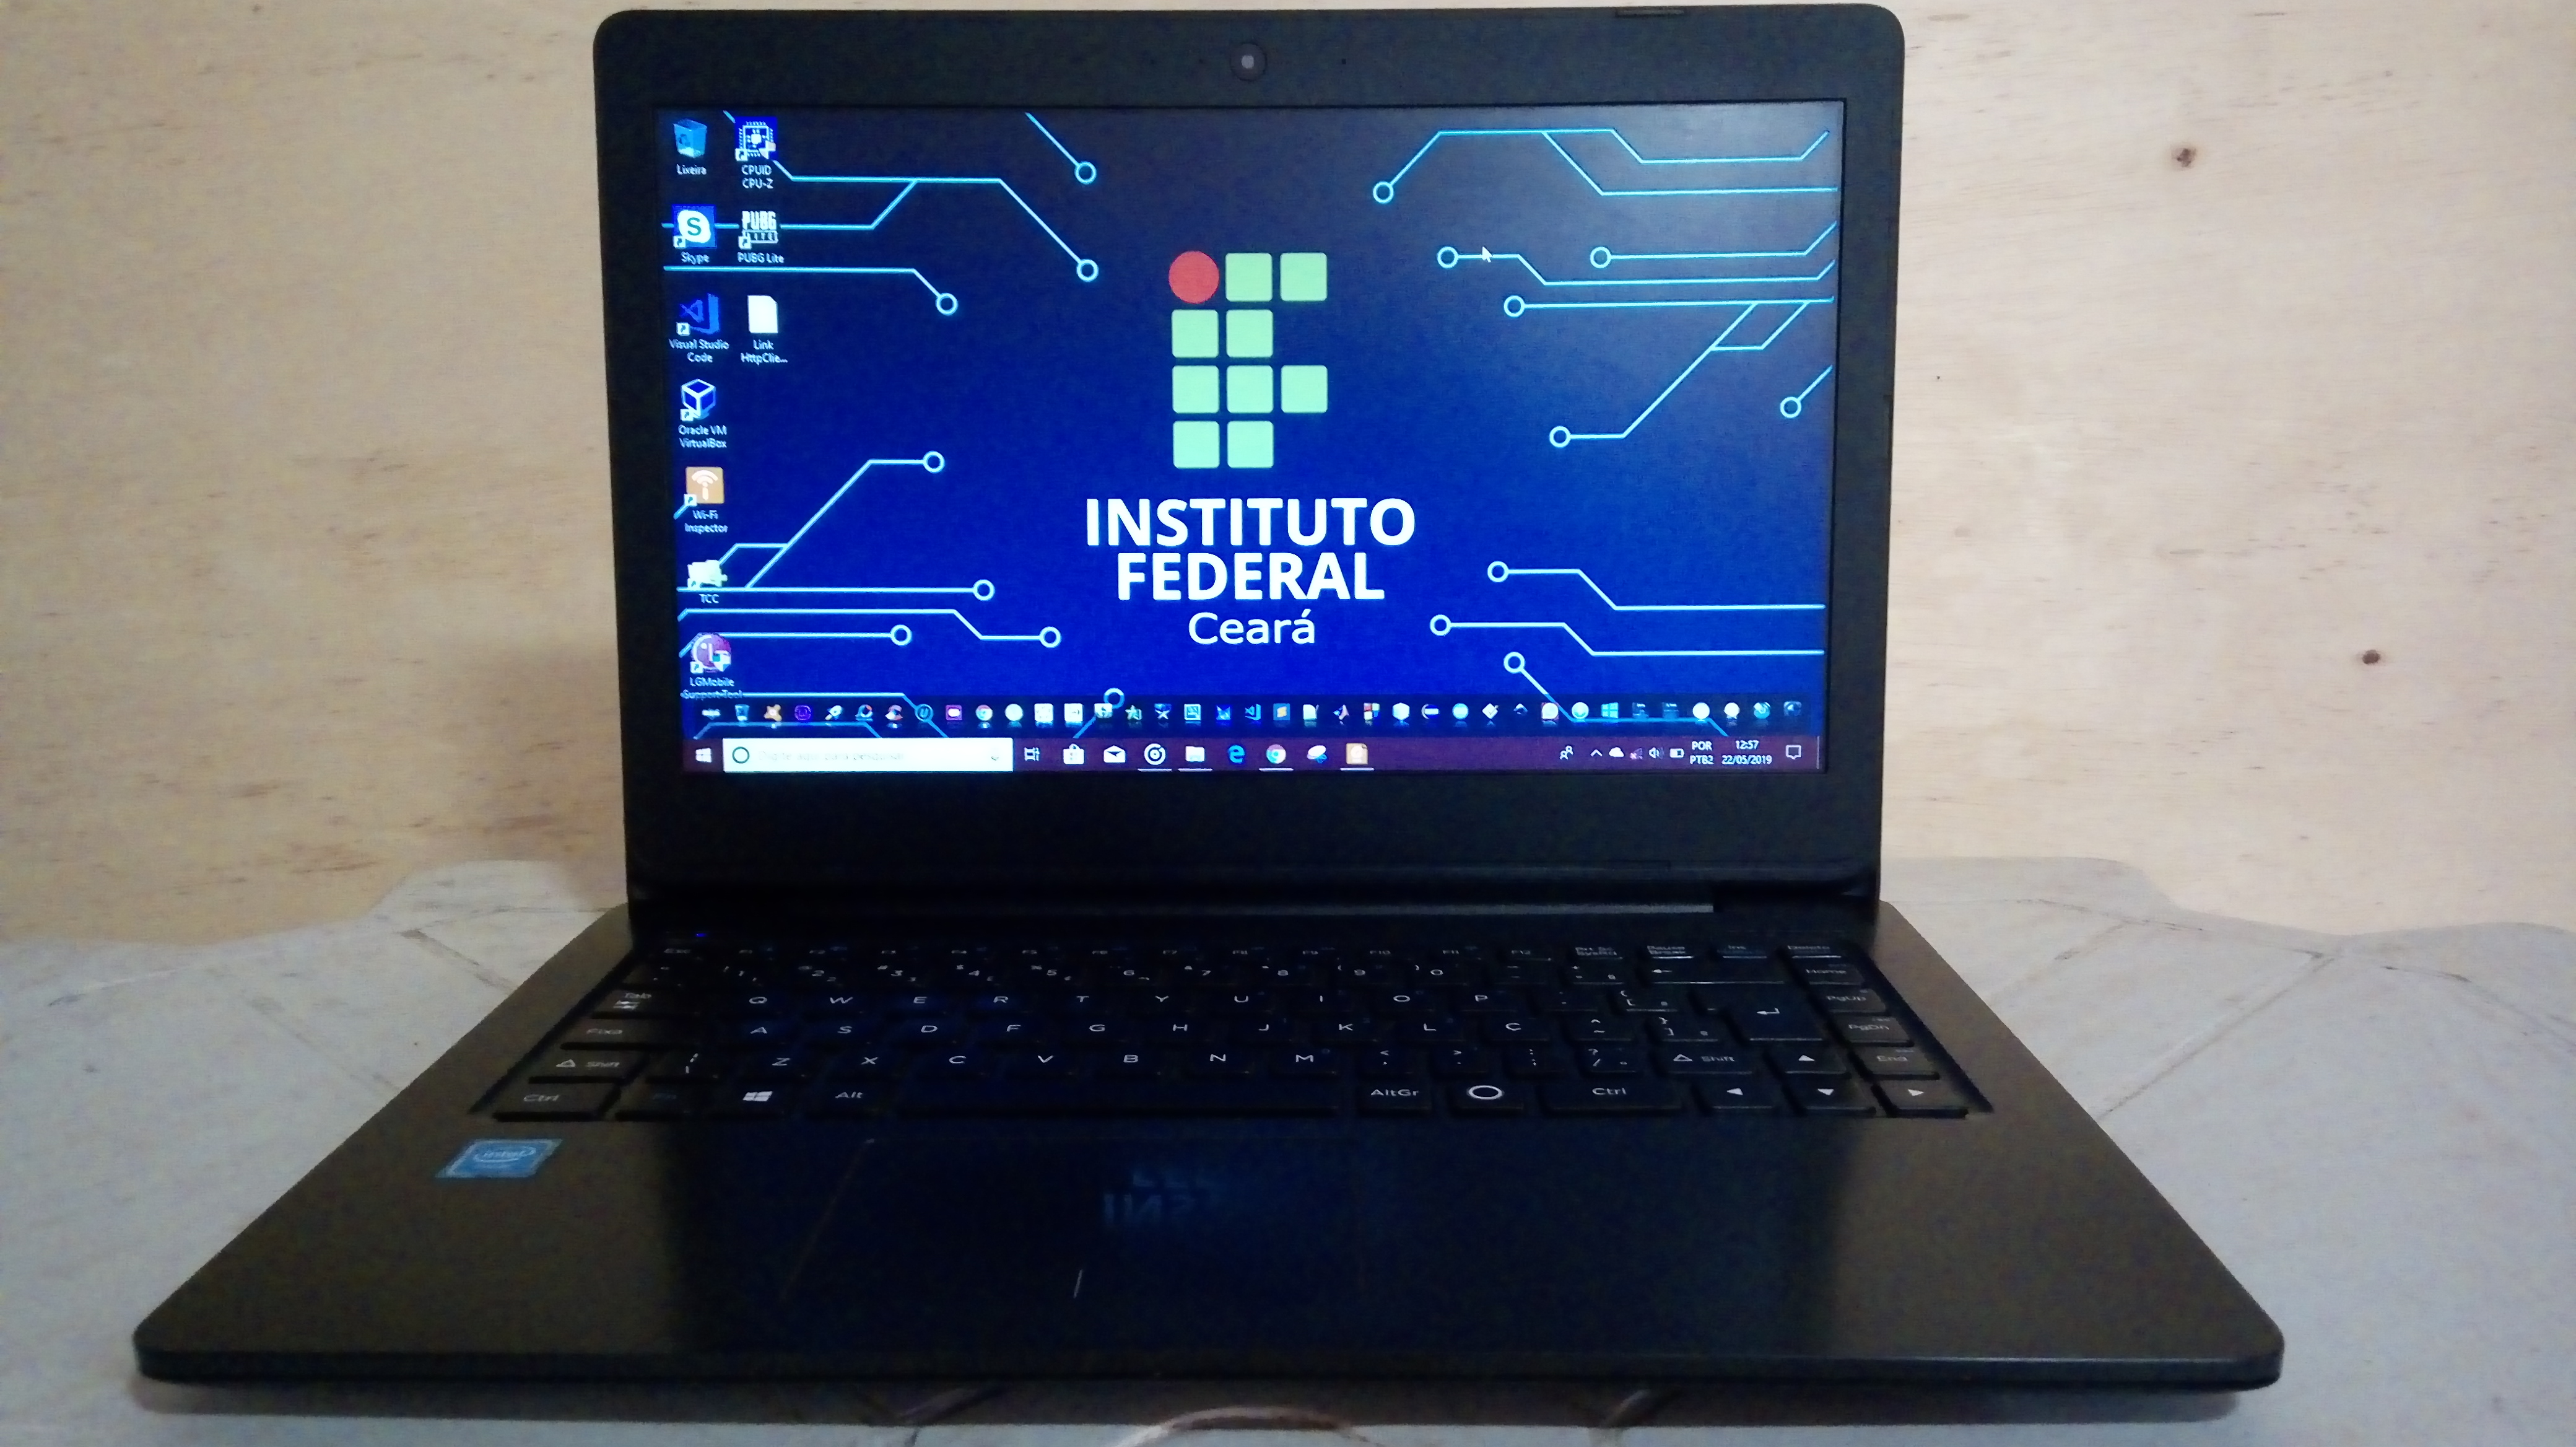
\includegraphics[scale=.1]{figuras/notebook.jpg}
	}{
		\Fonte{Autor.}%
	}	
\end{figure}

\begin{table}[H]
	\Caption{\label{tab:carac-notebook}Especificações do \textit{notebook} utilizado.}%
	\IBGEtab{}{%
		\begin{tabular}{ll}
			\toprule
			\multicolumn{1}{c}{Características do sistema} & \multicolumn{1}{c}{Descrição} \\
			\toprule %\midrule
			Modelo & Positivo Master N40i \\
			
			Sistema Operacional & Windows 10 Pro 64 bits \\
			
			Memória RAM & 4 GB \\
			
			Processador & Intel Celeron N3060 @1.60GHz (2 CPUs) \\
			
			Placa de rede & Intel Dual Band Wireless-AC 3160 \\
			\bottomrule
		\end{tabular}%
	}{%
		\Fonte{Autor.}%
	}%
\end{table}

\section{Execução do site survey}
\label{sec:execucao-site-survey}

O processo de \textit{site survey} desenvolvido no IFCE \textit{campus} Tauá, caracterizado como do tipo \textit{indoor}, foi dividido, para uma melhor execução, em quatro etapas que vão desde o início da coleta dos dados em campo até os resultados obtidos, definidas como se segue:

\begin{compactenum}
	\item Reconhecimento do local;
	\item Coleta dos dados;
	\item Tratamento dos dados;
	\item Geração dos mapas de calor.
\end{compactenum}

\subsection{Reconhecimento do local}
\label{subsec:reconhecimento-do-local}

Nesta primeira etapa do \textit{site survey}, após a instalação dos programas no \textit{notebook}, já citados, foi feita uma vistoria em toda a área correspondente ao Bloco Didático do \textit{campus} com a objetivo de verificar a sua infraestrutura física, identificar possíveis pontos para a medição e a presença ou não de fontes de interferências.

O ambiente analisado abrange uma área do tipo \textit{indoor} por conter salas, e também \textit{outdoor} devido ao espaço livre no prédio, como os que estão no térreo. O elevador, localizado no centro do prédio, como pode ser visto na imagem do topo da \autoref{fig:andar1} tem seu uso restrito à pessoas com necessidades especiais. Envolto ao elevador, a escadaria oferece o acesso aos dois pisos da construção. As Figuras \ref{fig:andar1} e \ref{fig:andar2} mostram alguns dos pontos que foram verificados.

\begin{figure}[H]
	\centering
	\Caption{\label{fig:andar1}Alguns dos locais inspecionados no térreo do Bloco didático.}	
	\UECEfig{}{
		\includegraphics[scale=.18]{figuras/Andar01.png}
	}{
		\Fonte{Autor.}%
	}	
\end{figure}

\begin{figure}[H]
	\centering
	\Caption{\label{fig:andar2}Alguns dos locais inspecionados no 1º andar do Bloco Didático.}	
	\UECEfig{}{
		\includegraphics[scale=.12]{figuras/Andar02.png}
	}{
		\Fonte{Autor.}%
	}	
\end{figure}

\subsection{Coleta dos dados}
\label{subsec:coleta-de-dados}

Nesta etapa foi iniciado o procedimento de medição dos níveis de potência, com a finalidade de obter informações das redes sem fio no \textit{campus} Tauá, sobretudo da cobertura das mesmas. O acesso e a utilização da planta baixa do Bloco Didático favoreceram para que fosse possível identificar a localização dos pontos de acesso e a estrutura física da instituição.

No Ekahau HeatMapper foi carregada a imagem da planta baixa do Bloco Didático. Logo após essa configuração, foi iniciada a demarcação dos pontos de medição por todo o local.

As primeiras medições ocorreram nos ambientes do tipo \textit{indoor} do Bloco Didático, o que inclui salas e laboratórios. Após a coleta dos níveis do sinal da rede de toda a parte interna, foi feita a captura na parte externa, como os corredores e locais sociais frequentados pelos estudantes. Em todo o prédio foram primeiramente analisados o térreo, e posteriormente o primeiro.

Para que todos os valores de medição obtidos na coleta fossem os mais precisos possível, foi feita uma comparação entre o ponto da planta baixa no Ekahau HeatMapper e o local da área real. Com isso, toda vez que um ponto de medida foi gerado, se obteve as potências de todas as redes Wi-Fi que estavam ao alcance do \textit{notebook}.

As medições ocorreram em 18 de maio de 2019 (sábado), pelo fato de que nesta data todos os docentes e discentes estariam ausentes do \textit{campus}. Isso contribuiu para que todas as salas e áreas que o Bloco Didático dispõe fossem visitadas e mapeadas.

A \autoref{fig:pontos-andar2} mostra os 62 pontos marcados no térreo do Bloco Didático. Cada ponto vermelho na figura significa um local que foi medido a potência de sinal da rede Wi-Fi. Já a \autoref{fig:pontos-andar1} apresenta todos os 50 pontos que foram medidos no térreo do mesmo prédio. Para cada ponto de medição, um tempo entre 30 e 60 segundos foi gasto com a finalidade de gerar um valor médio para a potência recebida naquele determinado ponto, pois o sinal sem fio sofre com flutuações rápidas, logo seu valor instantâneo pode não condizer com a realidade do local de medição.

\textcolor{blue}{A quantidade de pontos medidos nos dois andares compreende suficientemente toda a área útil do prédio. A localização de cada ponto procurou quantificar a potência do sinal em todos os locais com diferentes condições arquitetônicas para assim tornar os resultados os mais completos e precisos possíveis.}

\begin{figure}[H]
	\centering
	\Caption{\label{fig:pontos-andar2}Pontos de medida no 1º andar do Bloco Didático.}	
	\UECEfig{}{
		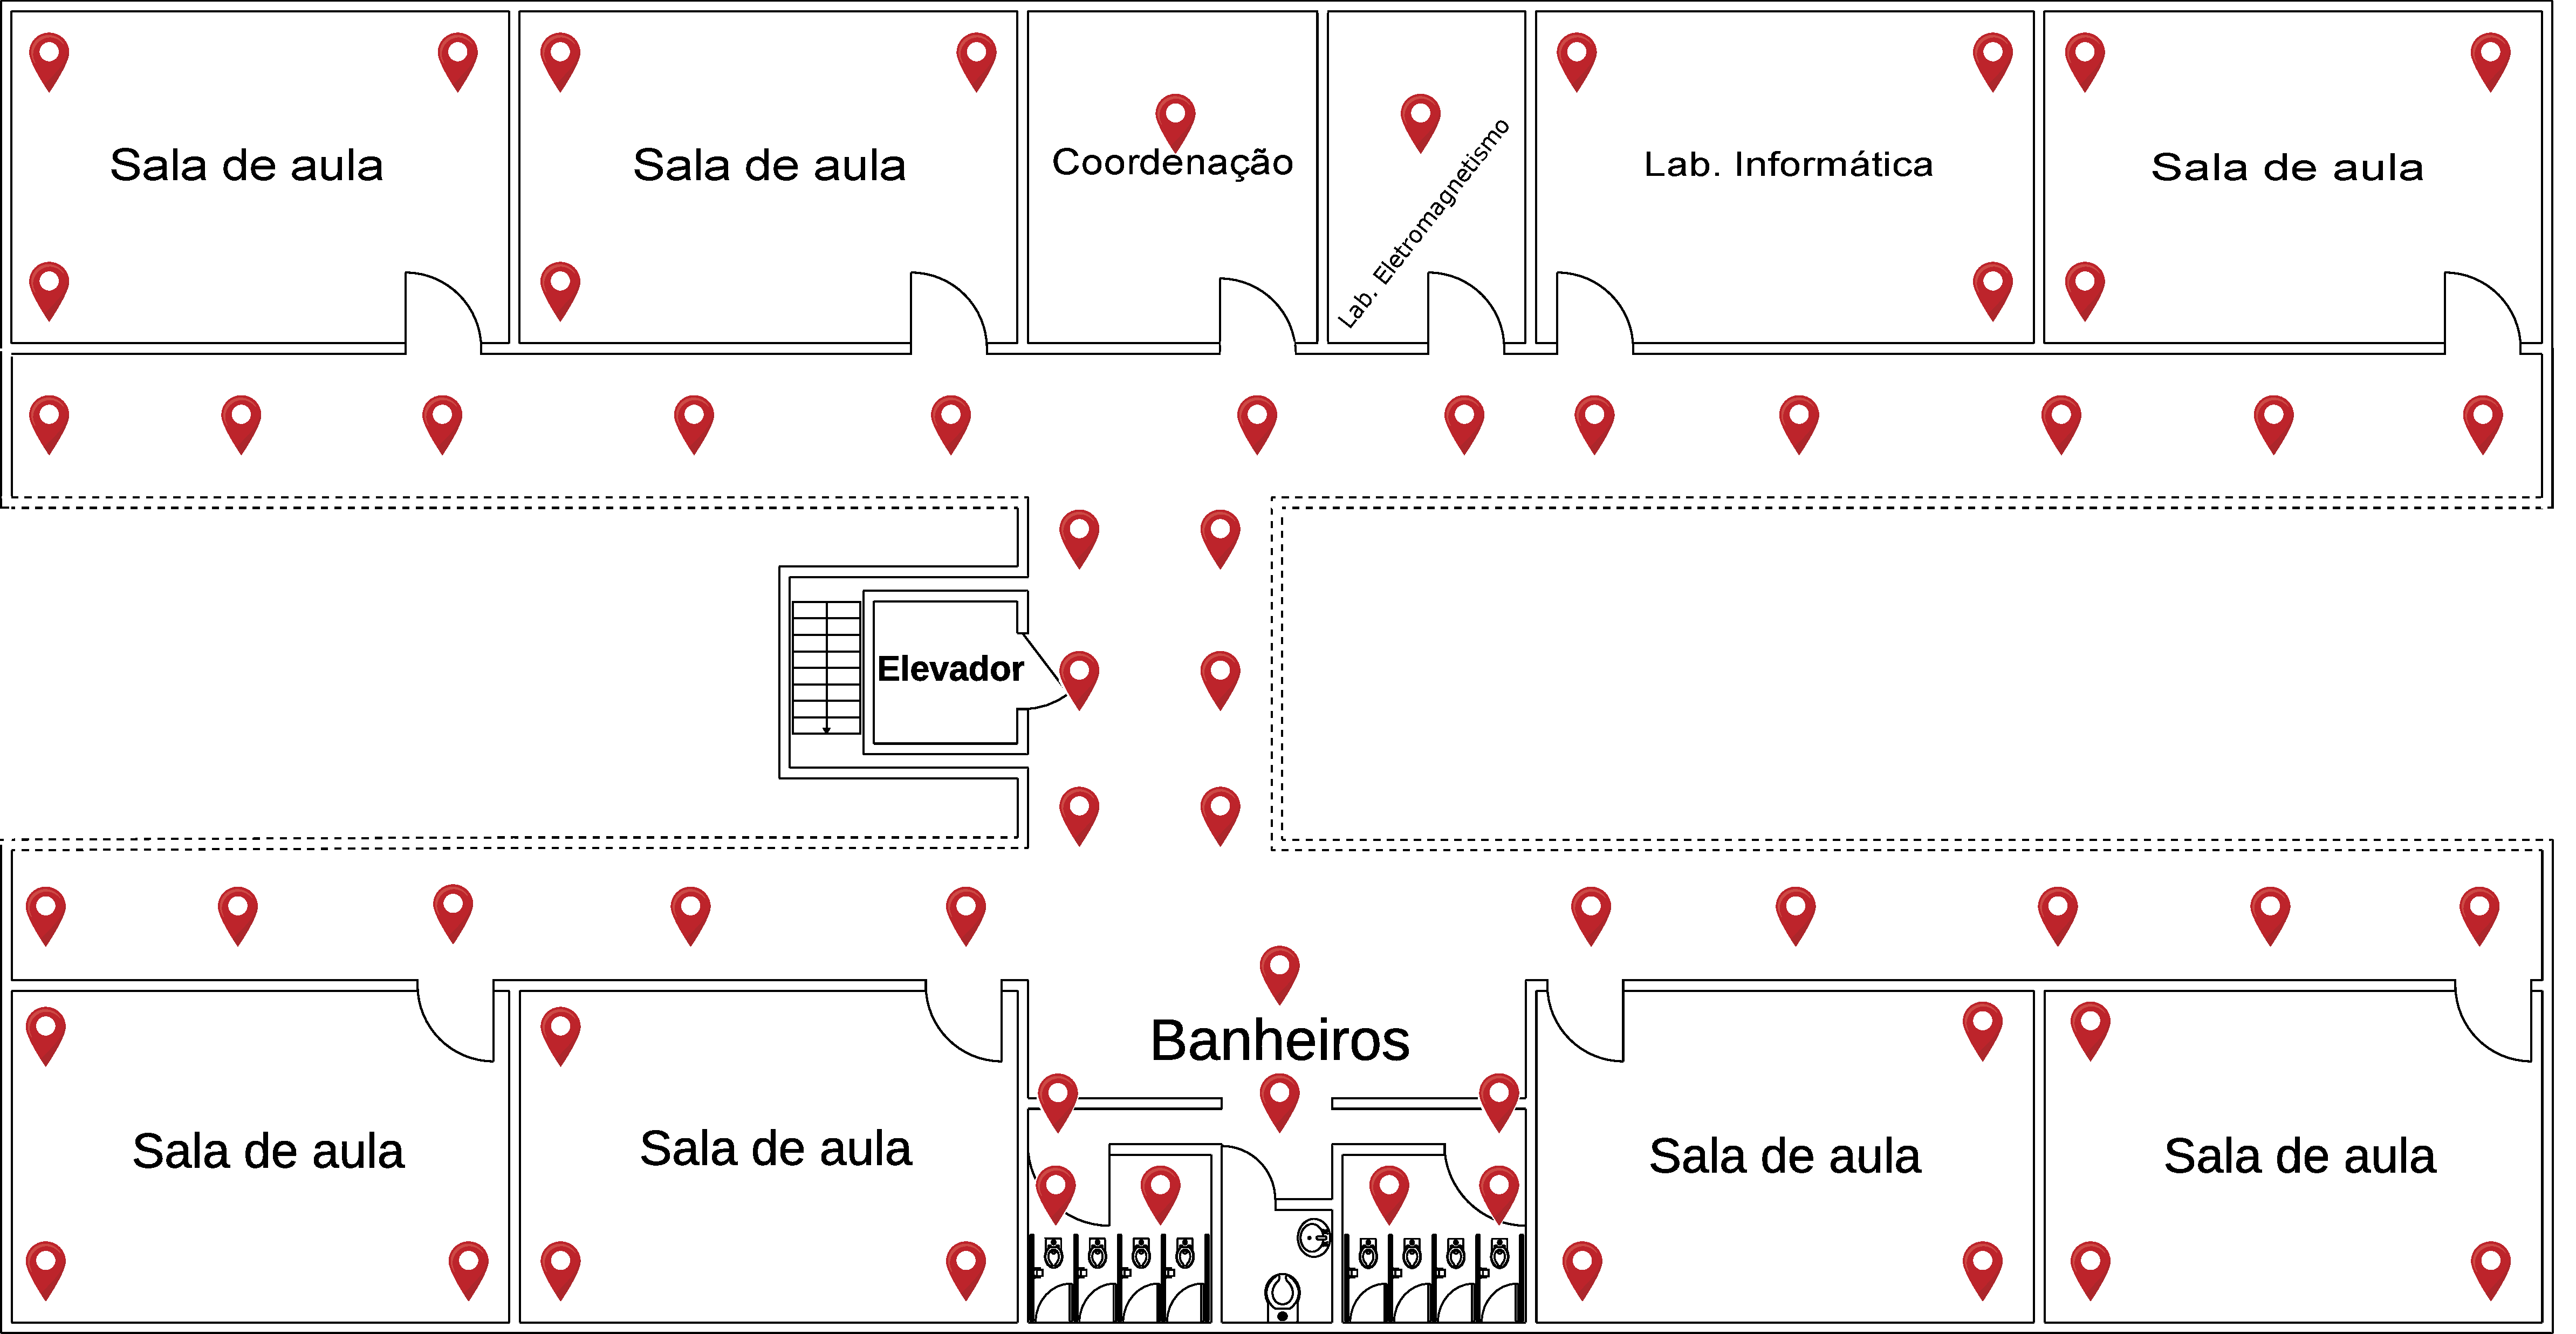
\includegraphics[scale=.2]{figuras/Pontos_Medidos_Andar02.pdf}
	}{
		\Fonte{Autor.}%
	}	
\end{figure}

\begin{figure}[H]
	\centering
	\Caption{\label{fig:pontos-andar1}Pontos de medida no térreo.}	
	\UECEfig{}{
		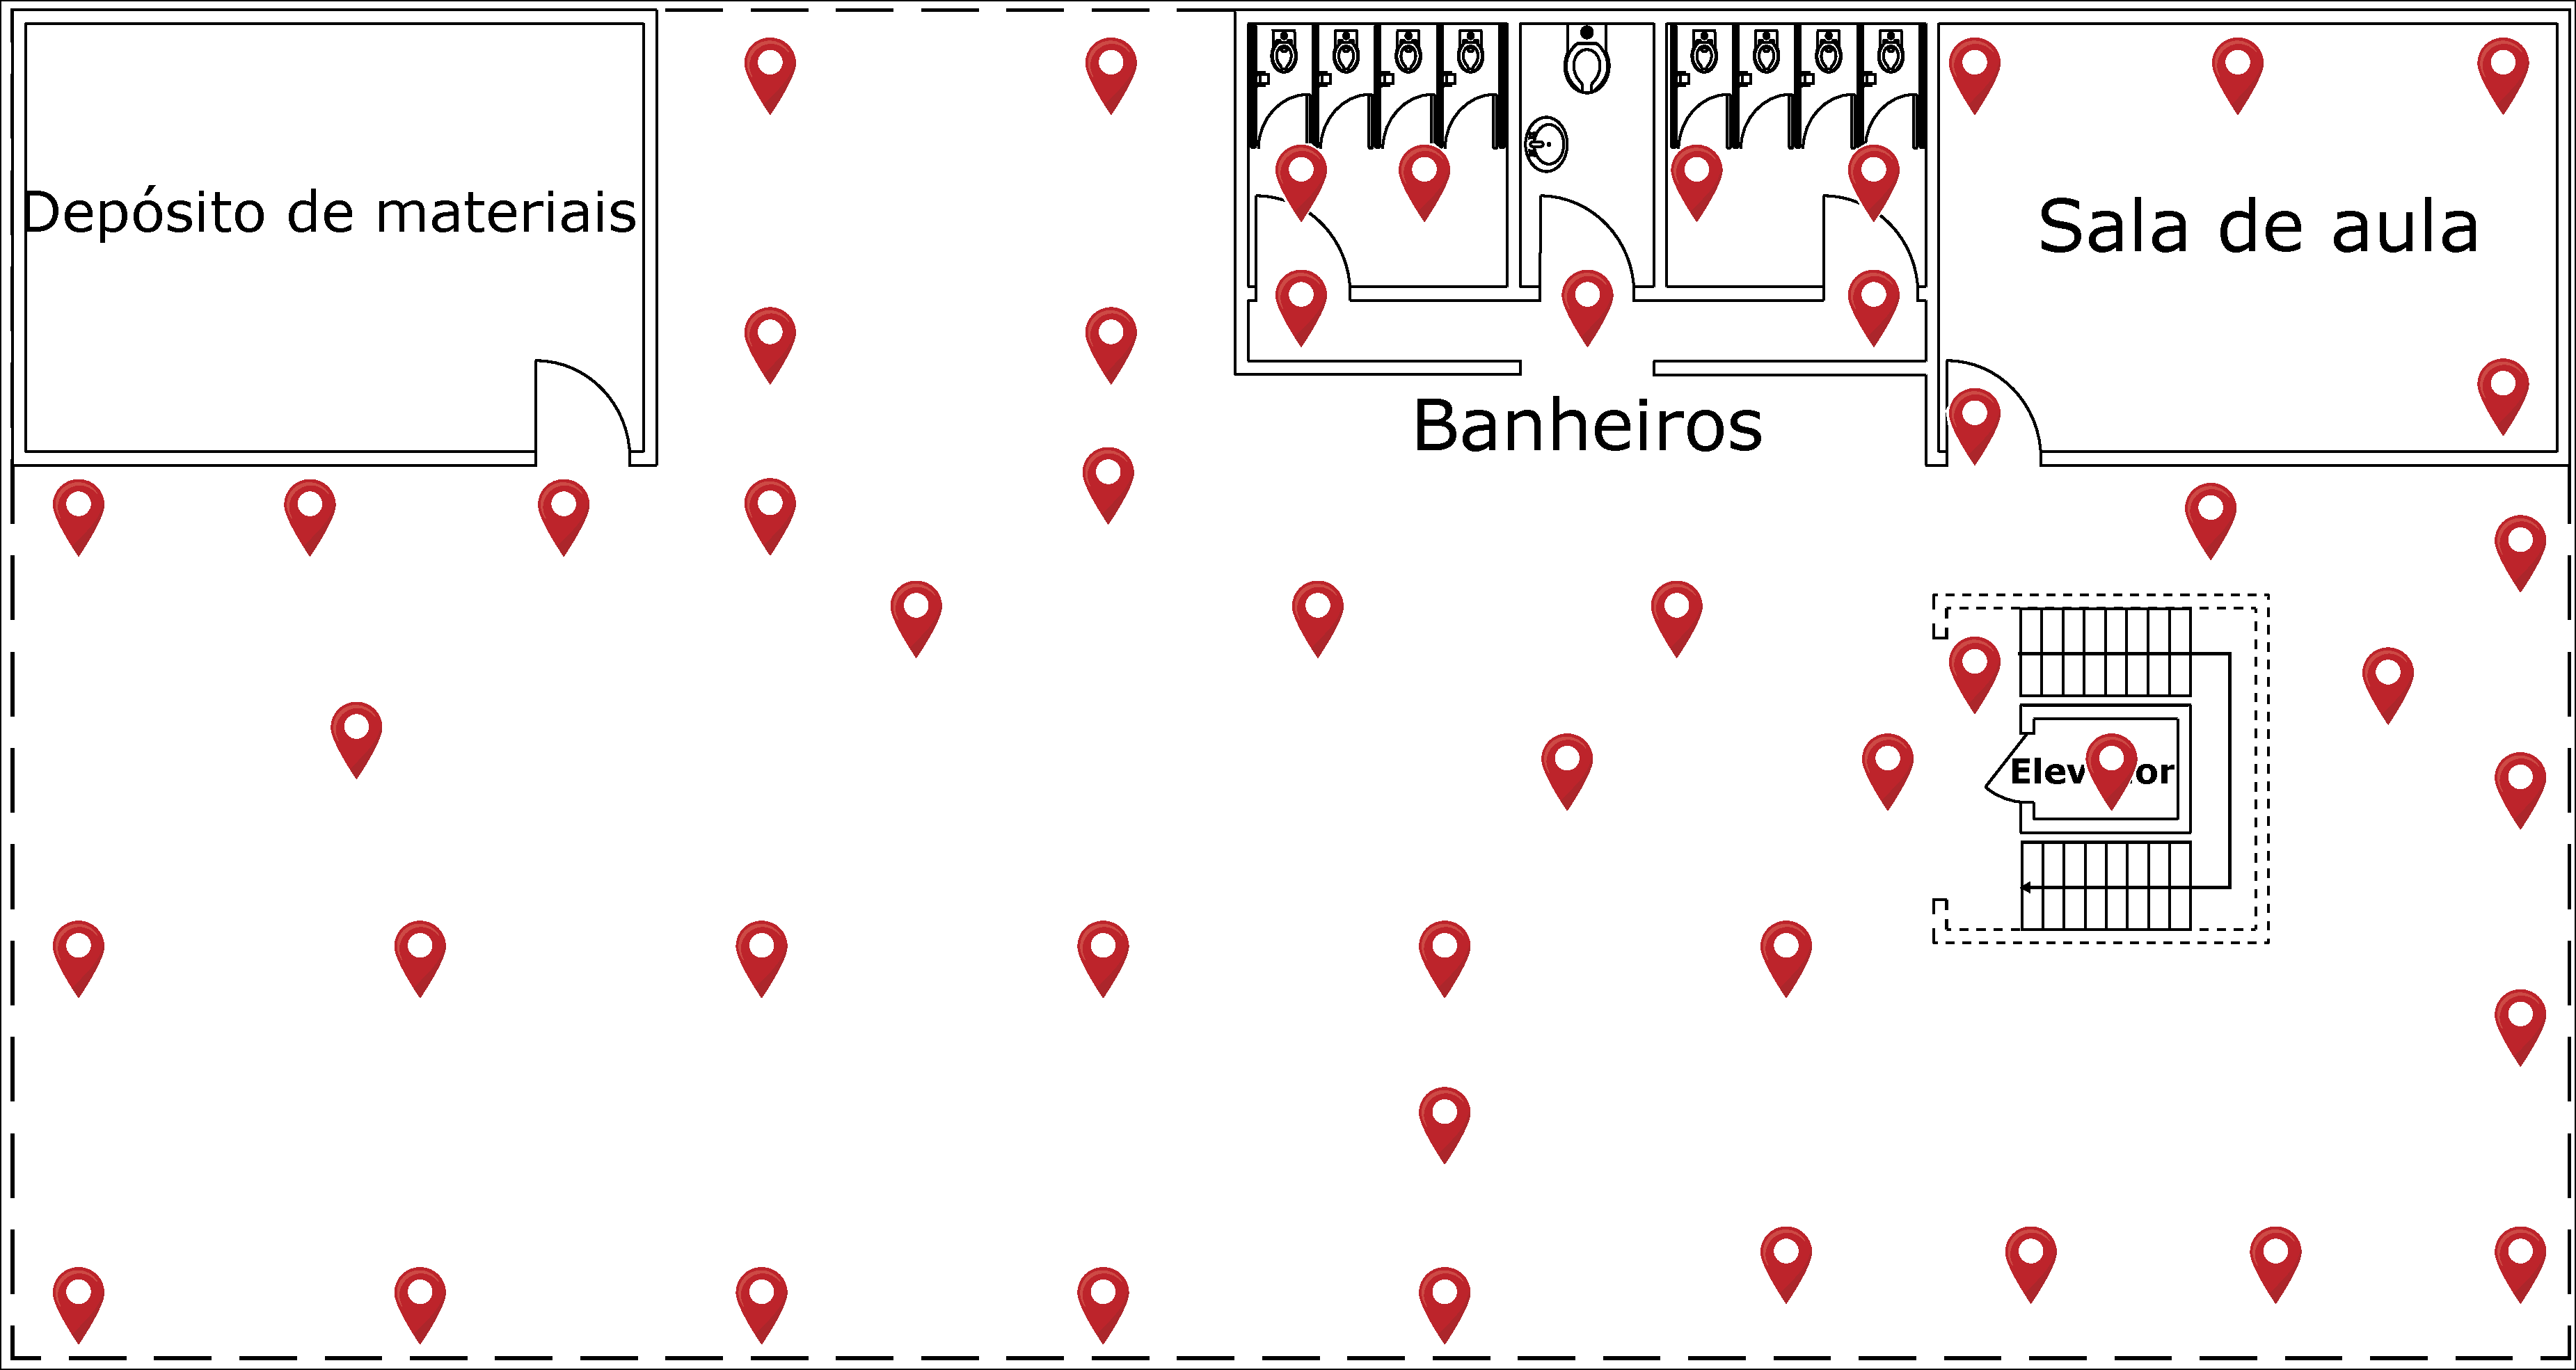
\includegraphics[scale=.25]{figuras/Pontos_Medidos_Andar01.pdf}
	}{
		\Fonte{Autor.}%
	}	
\end{figure}

\subsection{Tratamento dos dados}
\label{subsec:tratamento-dos-dados}

Após a coleta dos dados das redes sem fio detectadas no Bloco Didático, iniciou-se a etapa de tratamento dos mesmos, no qual foram analisados e depois utilizados filtros para definir quais dados das redes capturadas seriam aproveitados. \textcolor{blue}{Com o auxílio do Xirrus Wi-Fi Inspector, foram selecionadas informações que indicassem a frequência de operação e o canal utilizado pelos pontos de acesso com o objetivo de identificar interferências entre redes dentro da mesma área de cobertura.}

A \autoref{fig:networks-didatico} mostra a lista criada no Xirrus Wi-Fi Inspector com as características dos pontos de acessos detectados na varredura no térreo do Bloco Didático. A princípio, ao ser gerada a lista, são exibidos o SSID e o nível do sinal das redes, e também são disponibilizadas informações como canal, protocolo de segurança, padrão 802.11 utilizado e o fabricante do equipamento.

\begin{figure}[H]
	\centering
	\Caption{\label{fig:networks-didatico}Redes Wi-Fi detectadas pelo Xirrus Wi-Fi Inspector.}	
	\UECEfig{}{
		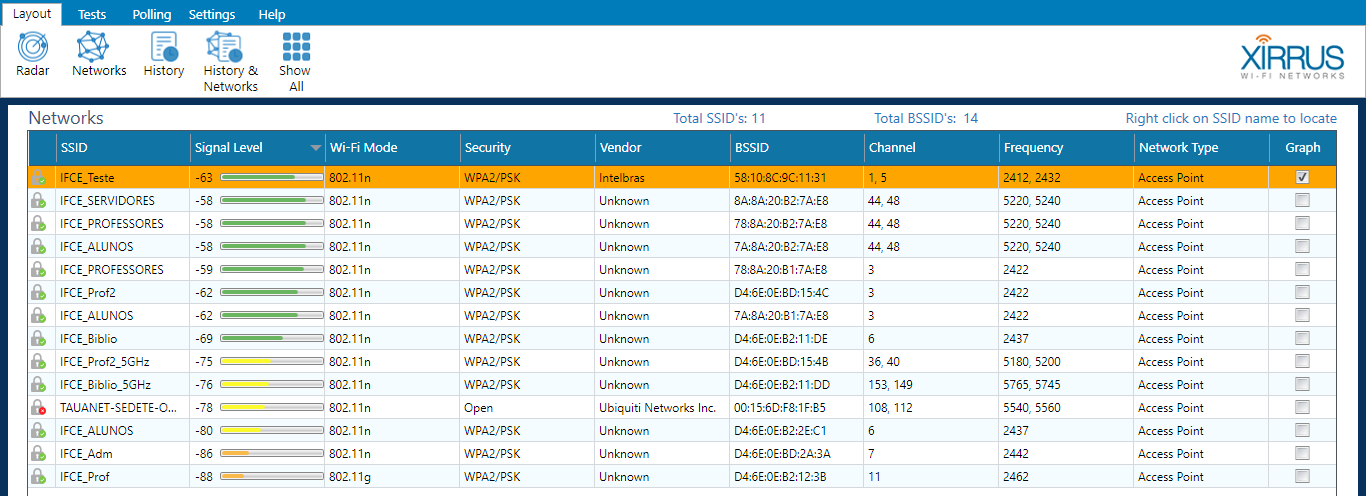
\includegraphics[scale=.43]{figuras/networks_didatic_recorte.png}
	}{
		\Fonte{Autor.}%
	}	
\end{figure}

\subsection{Geração dos mapas de calor}
\label{subsec:mapas-de-calor}

Ao final da etapa de tratamento de dados, a última fase do processo de \textit{site survey} é a geração dos mapas de calor da rede estudada.

Um mapa de calor é uma representação gráfica de dados em que os valores são representados como cores com significados determinados. Em redes sem fio, podem ser utilizados para gerar um mapa da cobertura da intensidade do sinal em toda a área de interesse, o que favorece uma análise mais visual e simplificada do ambiente \textit{wireless}. Nesse sentido, são amplamente recomendados para a demonstração dos resultados obtidos em um \textit{site survey}.

Os mapas de calor no Ekahau HeatMapper são gerados a partir da coloração entre várias cores como verde, amarelo, laranja e vermelho, que são utilizadas para representar as intensidades da potência recebida em um determinado ponto.

A \autoref{fig:escala-sinal} demonstra a barra de potência do Ekahau HeatMapper que pode receber uma variação de cores desde o verde ao vermelho.

\begin{compactitem}
	\item \textbf{Verde:} significa que o sinal recebido é muito forte.
	\item \textbf{Amarelo:} significa que a potência recebida é razoável.
	\item \textbf{Laranja:} significa que a potência obtida é ruim.
	\item \textbf{Vermelho:} significa que a potência do sinal recebido é muito fraco.
\end{compactitem}

\begin{figure}[H]
	\centering
	\Caption{\label{fig:escala-sinal}Escala de potência do sinal.}	
	\UECEfig{}{
		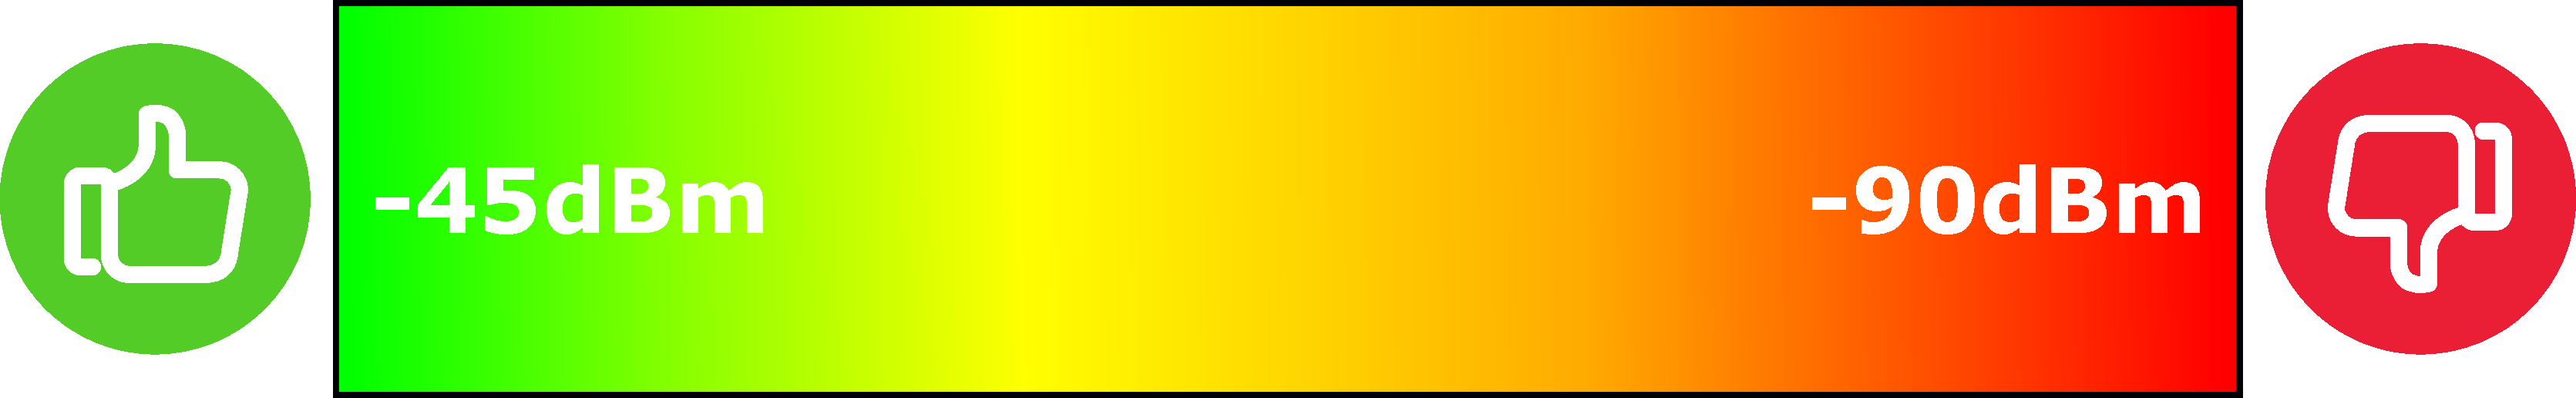
\includegraphics[scale=.185]{figuras/Escala_dBm.pdf}
	}{
		\Fonte{Autor.}%
	}	
\end{figure}

Para que os mapas fossem gerados, foram definidos valores de potência baseados em testes de distância entre um ponto de acesso e o \textit{notebook}, no qual --85dBm (ou menor) representa uma área de sombra, isto é, sem propagação suficiente de sinal, e no mapa aparecerá a tonalidade mais forte de vermelho. Isso significa que toda área do mapa que receber esse nível de sinal será considerada de perda de conectividade. Caso a potência recebida no mapa for de --45dBm (ou maior, caso o receptor seja capaz de detectá-la), isto significa que o local mapeado possui alta conectividade, sendo assim representada pela cor verde.

\section{Resultados do Site Survey}
\label{sec:resultados-site-survey}

Com a ferramenta de \textit{software} Ekahau HeatMapper foram gerados dois mapas de calor, ambas da rede Wi-Fi do Bloco Didático, o que inclui os dois pontos de acesso instalados no local. A seguir são demonstrados os resultados obtidos através da aplicação da metodologia de \textit{site survey} realizado na área já mencionada.

Por questões de autorização, apenas na rede destinada aos discentes (SSID IFCE\_Teste) foram feitos os mapas de calor. Pelo fato do ponto de acesso atribuído aos docentes (SSID IFCE\_PROFESSORES) estar localizado próximo ao dos estudantes na sala de coordenação, os mapas de calor resultantes de ambas provavelmente seriam equivalentes, ou seja,  com o mapeamento de apenas uma das redes o mesmo resultado se aplicaria a outra com margem de erro desprezível para caso de verificação da propagação de radiofrequência.

A \autoref{fig:heatmapper-andar2} apresenta visualmente o mapa de calor da rede IFCE\_Teste para o térreo do Bloco Didático, e o maior nível de potência que é recebido é representado por verde e o menor nível de potência recebido é definido pela cor vermelha. Cada pequeno ponto\footnote[6]{Por algum motivo, o programa Ekahau HeatMapper não exibiu certos pontos medidos. No entanto, não houve prejuízos significativos ao resultado final do mapeamento.} verde interligado a outro por um segmento de reta representa o local onde foi efetuada uma medição de sinal.
\newpage
\begin{figure}[H]
	\centering
	\Caption{\label{fig:heatmapper-andar2}Mapa de calor da rede IFCE\_Teste para o 1º andar do Bloco Didático.}	
	\UECEfig{}{
		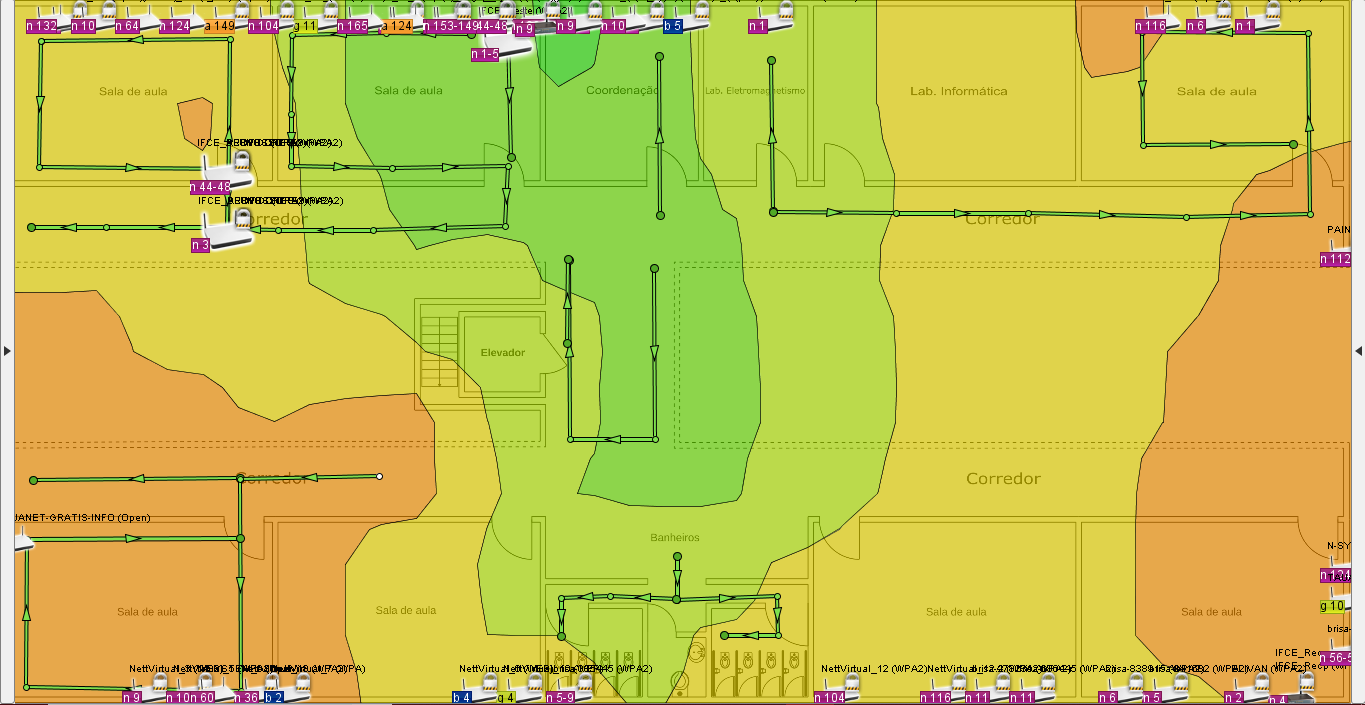
\includegraphics[scale=.65,angle=90]{figuras/heatmapper_2_andar.png}
	}{
		\Fonte{Autor.}%
	}	
\end{figure}

Como se pode observar pela área do mapa de calor da \autoref{fig:heatmapper-andar2}, as regiões que apresentaram maiores níveis de intensidade de sinal de rádio favoráveis para uma conexão foram as áreas localizadas nas imediações do centro da planta baixa, destacadas pelos tons de verde, e também pelas partições adjacentes a sala de coordenação.

Nota-se que os sinais propagados pelo térreo sofrem algumas atenuações como por exemplo nos extremos direito e esquerdo do mapa em que a coloração alaranjada simboliza locais com considerável perda de potência. Levando em consideração, pelo mapa, que as áreas mais afetadas pela perda de conectividade são as salas de aula e os corredores, frequentadas diariamente por estudantes, é indispensável a implantação de novos pontos de acesso para suprir esses locais onde o sinal perde força.

A \autoref{fig:heatmapper-andar1} representa o mapa de propagação de sinal do térreo do Bloco Didático para a rede IFCE\_Teste. A partir do mapa de calor gerado com as devidas colorações, nota-se que a rede mapeada não dispõe de uma área de cobertura que abrange todo o espaço do andar. Como é possível perceber, na maior parte do mapa as áreas apresentam tons de cor mais ``quentes'', o que significa que o ambiente não recebe bons níveis de potência de rádio para o estabelecimento de uma conexão de dados confiável. No depósito não foram realizadas medições pelo fato de o local ser usado simplesmente para armazenamento de materiais.

Logo, para que a rede IFCE\_Teste tenha uma cobertura de sinal por todo o térreo, seria necessário futuramente acrescentar mais equipamentos de acesso que irradiem sinais que alcancem as zonas com deficiência de propagação de rádio.

\begin{figure}[H]
	\centering
	\Caption{\label{fig:heatmapper-andar1}Mapa de calor da rede IFCE\_Teste para o térreo do Bloco Didático.}	
	\UECEfig{}{
		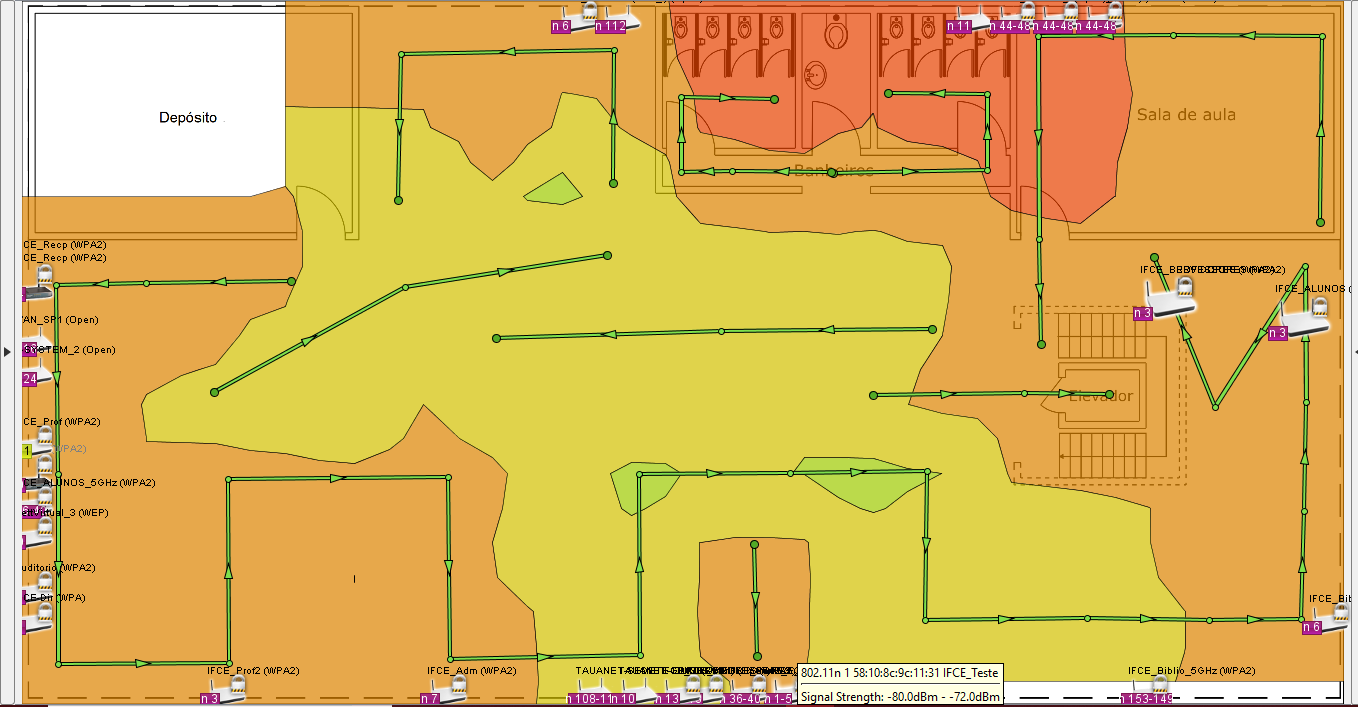
\includegraphics[scale=.64,angle=90]{figuras/heatmapper_Terreo_Editada.png}
	}{
		\Fonte{Autor.}%
	}	
\end{figure}


\section{Discussão dos Resultados}
\label{discussao-dos-resultados}

Os resultados encontrados no presente estudo evidenciam que a metodologia \textit{site survey} contribuiu significamente na avaliação da qualidade do sinal da rede Wi-Fi do Bloco Didático do IFCE Tauá, demonstrando que os dois andares mapeados apresentam níveis de propagação de radiofrequência distintos. Isso se deve ao fato de cada um dos andares possui diferentes estruturas arquitetônicas, o que influencia diretamente no alcance máximo de cada célula instalada.
	
Existem dois pontos de acesso disponíveis exclusivamente para atender o prédio, sendo um destinado aos docentes e o outro aos discentes, ambos instalados no mesmo local (sala de coordenação). Por estarem tão próximos, a cobertura de cada ponto de acesso não é adequadamente distribuída pela área, as duas zonas de serviço se sobrepõem. Porém, não há problemas de interferência entre as redes Wi-Fi, já que a rede com SSID IFCE\_Teste opera na banda de frequência de 2.4 GHz e a rede com SSID IFCE\_PROFESSORES trabalha em 5 GHz, como mostra a captura de tela da \autoref{fig:networks-didatico}. Ainda na \autoref{fig:networks-didatico} percebe-se que a rede IFCE\_PROFESSORES pode sofrer com interferências de outras redes que operam na mesma faixa de frequência e se encontram instaladas no bloco principal do \textit{campus} mas que são detectadas no Bloco Didático.

No mapa de calor gerado para o térreo do Bloco Didático (\autoref{fig:heatmapper-andar2}) observa-se a predominância de tons de verde na região central do piso. Isso quer dizer que nesse local o nível de potência recebido é forte para o estabelecimento de conexões de alta velocidade com a Internet. A medida que a distância de análise aumenta em relação ao ponto de acesso, as cores mudam para amarelo e laranja informando que nesses pontos a qualidade do sinal Wi-Fi diminuiu consideravelmente. Se forem consideradas as áreas livres de barreiras, como os corredores, a atenuação sofrida pelo \textit{link} de rádio é gradual, causada pela perda de espaço livre durante o percurso. 

As regiões mais extremas do mapa são as que mais perdem sinal em função da distância até o ponto de acesso, principalmente a parte superior, entretanto, no canto inferior direito o formato da zona laranja difere bastante da superior direita. Nesse local a mancha de perda concentra-se quase que unicamente na sala de aula. Analisando a imagem, observa-se que entre o ponto de acesso e a referida zona existe a presença do elevador. Por ser constituído de metal, este obstáculo absorve grande parte da energia da onda de rádio, o que prejudica sua propagação. Além disso, por ser um ambiente \textit{indoor}, é importante ponderar as perdas causadas ao sinal pela penetração da ondas de rádio em paredes: quanto mais barreiras maior a degradação. O material utilizado na construção da parede também pesa contra a propagação eletromagnética.

Em contraste ao segundo piso, o térreo do Bloco Didático possui apenas uma sala de aula, uma sala de depósito de materiais e o elevador, o restante é área aberta de convívio social dos estudantes do \textit{campus}. Por esta última descrição, seria lógico supor que o mapa de calor obtido apresentasse bons níveis de potência de sinal recebido, no entanto, o resultado final foi totalmente oposto. Como pode ser visto na mapa de calor da \autoref{fig:heatmapper-andar1}, a propagação de rádio no térreo situa-se de ruim a péssima por não existir grande concentração de tons de verde no mapa, praticamente só as cores amarelo, laranja e vermelho. Como os pontos de acesso estão confinados no térreo, as ondas de rádio obrigatoriamente atravessam o piso de concreto armado, com espessura bem maior do que as paredes das salas. Isso significa que quando o sinal passa através deste obstáculo ele já chega muito atenuado no piso inferior. No local onde fica os banheiros o sinal é ainda pior devido a existência das paredes, o que torna a conexão com a rede extremamente lenta.

% Sugestão de intervenção na rede sem fio
Diante de todas as discussões feitas, infere-se que intervenções na rede sem fio do Bloco Didático seriam necessárias para que a distribuição da cobertura de sinal seja mais homogênea, o que provavelmente resultaria em um nível de desempenho satisfatório para os clientes.

Tomando como base o mapa de calor do térreo (\autoref{fig:heatmapper-andar2}), a principal recomendação seria acrescentar, no mínimo, outro ponto de acesso e deslocar para fora o que está na sala de coordenação, reposicionado-os próximos aos extremos do prédio. Aconselha-se configurar os pontos de acesso para que operem em 2.4 GHz, já que ondas de rádio nessa frequência podem passar através de paredes, pisos e tetos. Portanto, elas podem chegar em locais desejáveis. Assim, áreas antes sem cobertura de sinal poderão ter maiores chances de receberem níveis mais elevados de potência em relação a rede existente. Para evitar interferência destrutiva, os equipamentos devem ser configurados em canais diferentes, de preferência 1, 6 ou 11. O possível novo posicionamento dos pontos de acesso para a abordagem sugerida pode ser visto na \autoref{fig:proposta1}.

\begin{figure}[H]
	\centering
	\Caption{\label{fig:proposta1}Proposta de posicionamento dos pontos de acesso para o 1º andar do Bloco Didático.}	
	\UECEfig{}{
		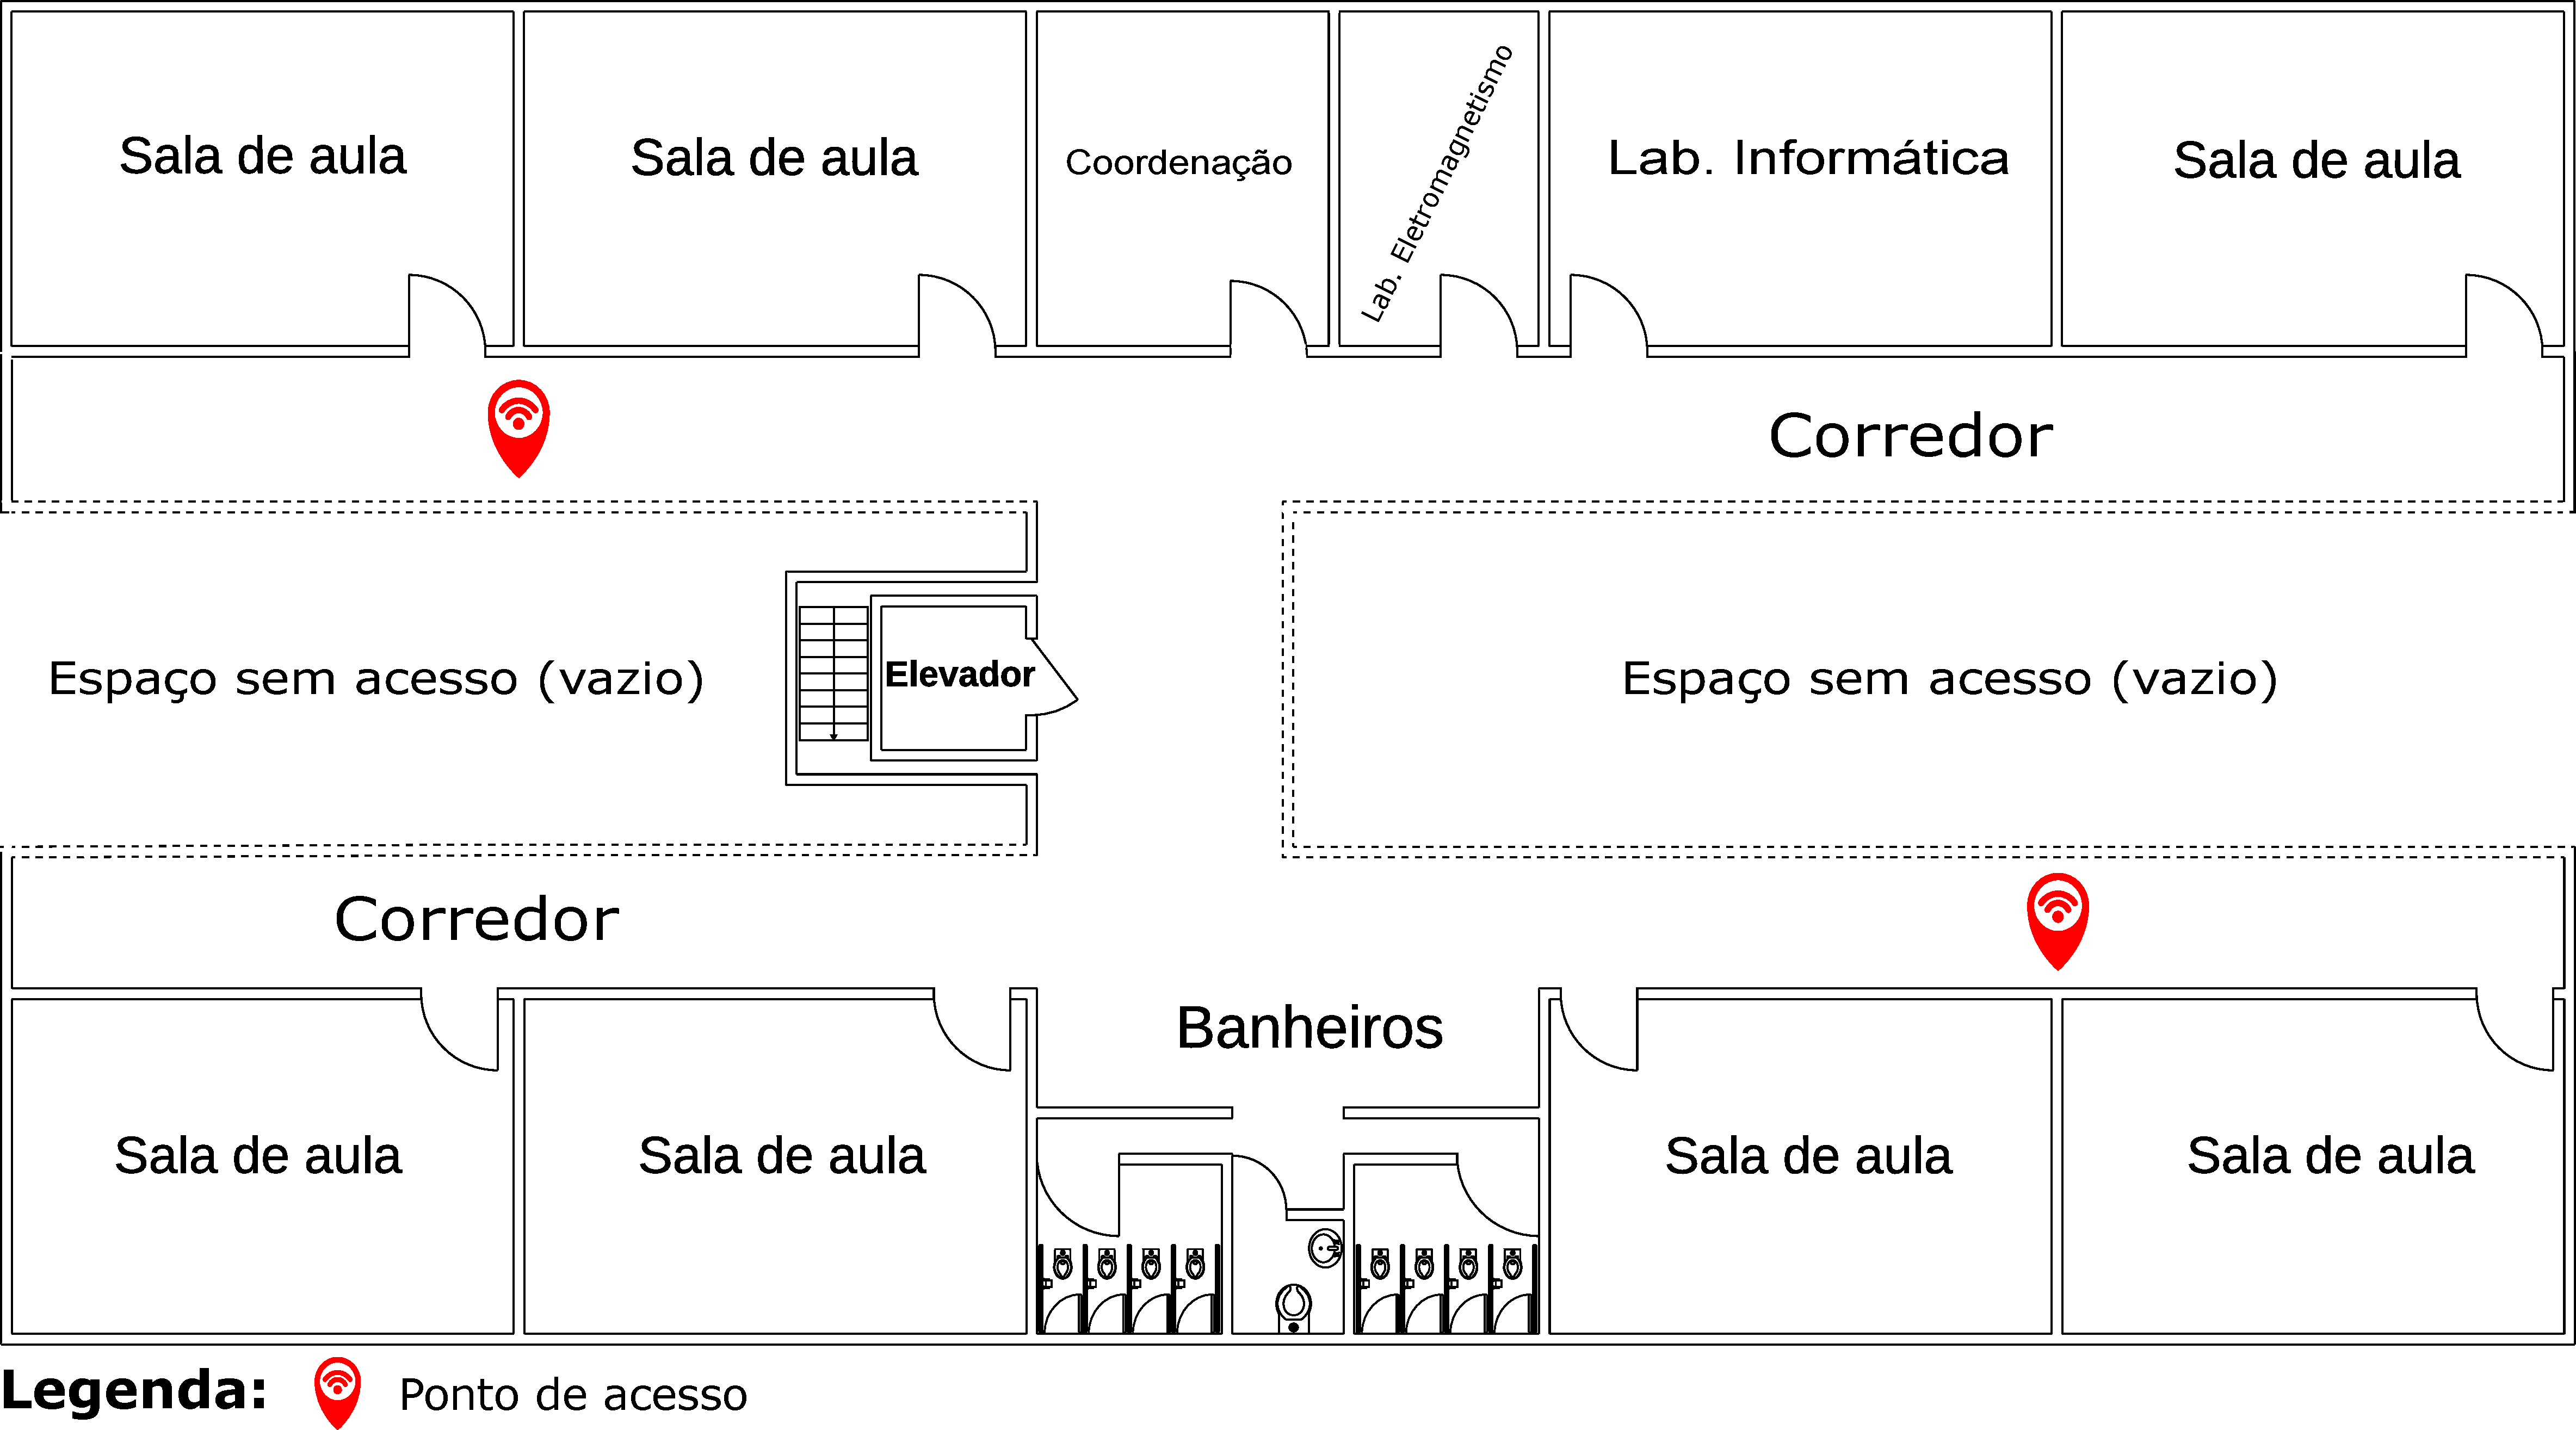
\includegraphics[scale=.18]{figuras/APs_Bloco_Andar_2_Proposta_Intervencao.pdf}
	}{
		\Fonte{Autor.}%
	}	
\end{figure}

Por não conter nenhum ponto de acesso, o térreo precisaria também de, no mínimo, dois equipamentos para prover condições satisfatórias de conexão de dados, como ilustra visualmente a  \autoref{fig:proposta2}. Ainda poderia ser utilizados pontos de acesso na frequência de 5 GHz, pois assim evitaria-se interferências com a rede do térreo (supondo que a recomendação feita tenha sido atendida), além de oferecer alta taxa de transmissão de dados em comparação com a ofertada pela banda de 2.4 GHz.

\begin{figure}[H]
	\centering
	\Caption{\label{fig:proposta2}Proposta de posicionamento dos pontos de acesso para o térreo andar do Bloco Didático.}	
	\UECEfig{}{
		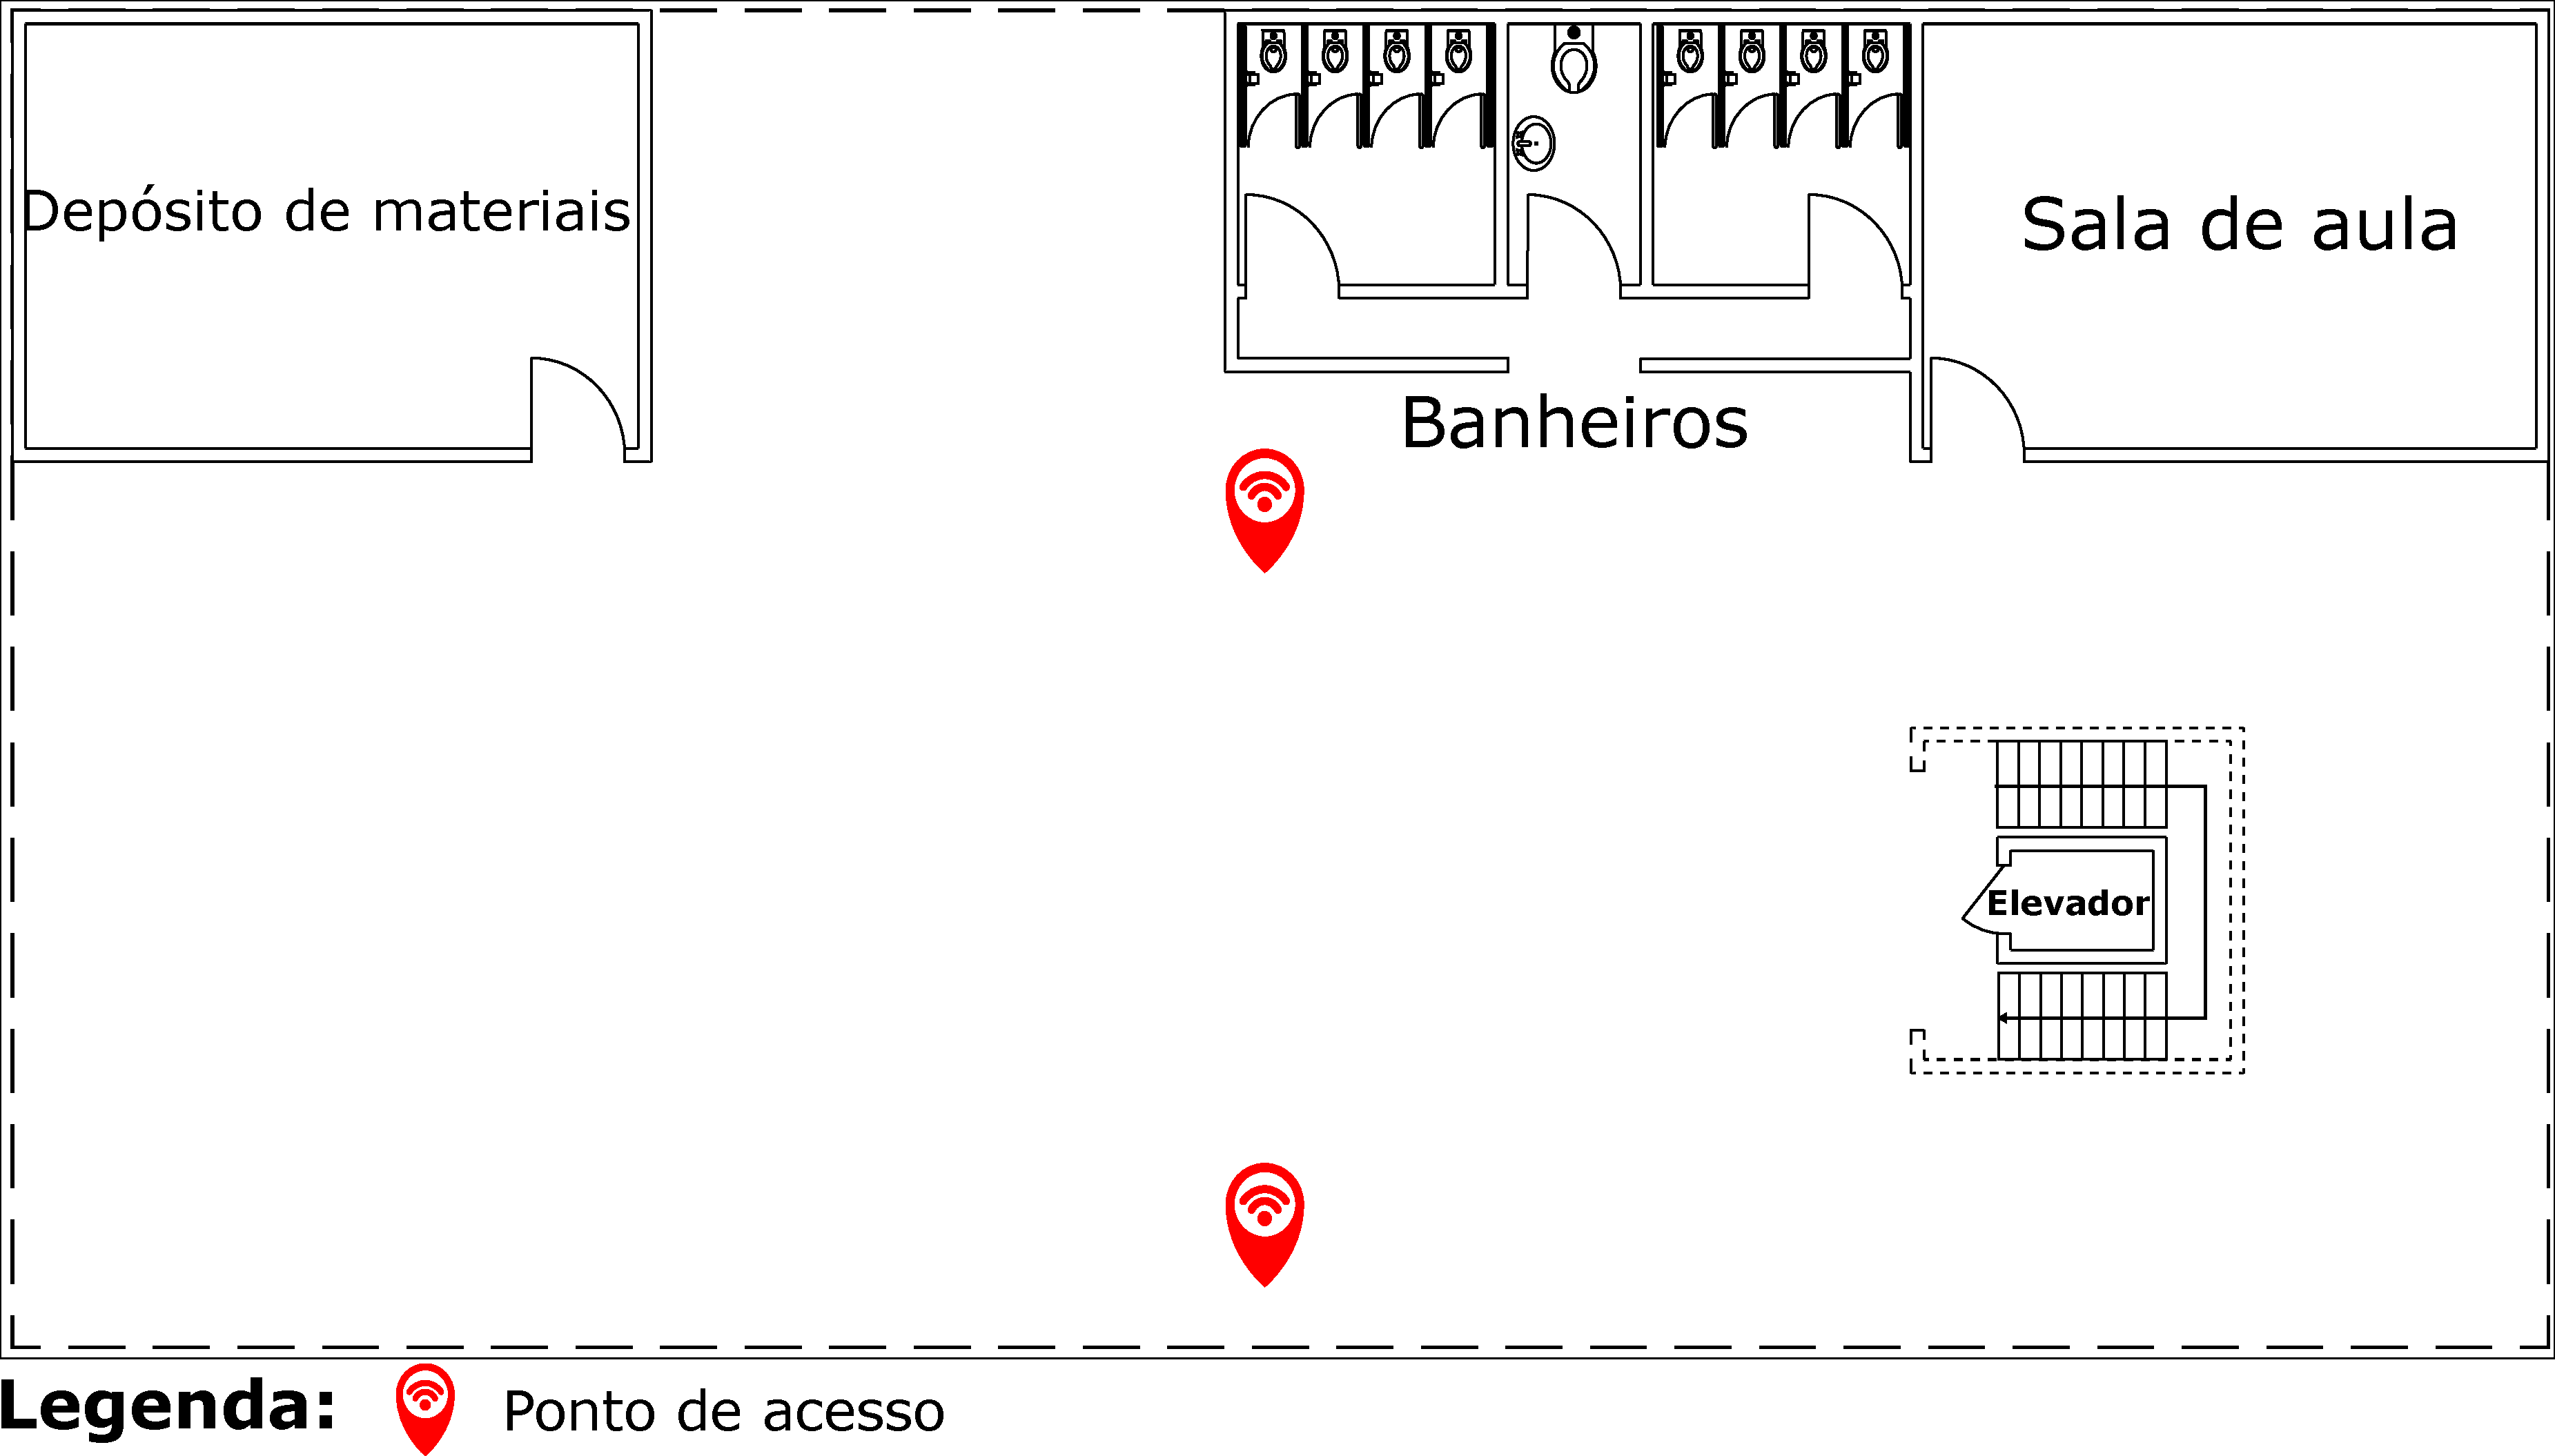
\includegraphics[scale=.22]{figuras/APs_Bloco_Andar_1_Proposta_Intervencao.pdf}
	}{
		\Fonte{Autor.}%
	}	
\end{figure}

A justificativa para as duas propostas descritas acima fundamenta-se na utilização de pontos de acesso com antenas omnidirecionais, ou seja, que irradiam radiofrequência em todas as direções a partir do ponto de origem, distribuindo o sinal por uma área maior, ao mesmo tempo que eleva o nível de potência recebido em pontos antes castigados com a baixa conectividade. Outro motivo é que cada andar possui condições estruturais diferentes um do outro. Isso contribui diretamente no posicionamento dos pontos de acesso a fim de proporcionar as melhores condições de propagação do sinal pelo prédio.